\chapter{Experimentação e Avaliação}
\label{chap:experimentacao}

Este capítulo tem como objetivo apresentar e discutir os resultados obtidos por meio dos painéis do ambiente analítico desenvolvido, evidenciando de que forma a integração entre o modelo de risco proposto, os dados institucionais e os dados históricos de mercado se traduzem em análises quantitativas sobre o conjunto de ações.

\section{Metodologia de Validação Cruzada com o S\&P 500}
\label{sec:validacao-sp500}

A validação do modelo proposto é conduzida por meio de comparação entre o desempenho histórico de carteiras construídas a partir do \textit{score} de risco descrito na Seção \ref{sec:modelagem-risco}, eventualmente combinado aos modificadores apresentados na Seção \ref{sec:modificadores}, e o desempenho do índice de referência adotado como \textit{benchmark}. O objetivo da etapa não é demonstrar superioridade absoluta do modelo, e sim verificar se a inclusão de cada modificador e de suas combinações altera o perfil de risco e retorno das carteiras resultantes quando confrontadas com o comportamento do mercado representado pelo \textit{benchmark}.

\subsection{\textit{Benchmark} Único de Comparação}

A escolha do índice de mercado contra o qual o modelo é avaliado constitui parte do \textit{setup} experimental e impacta diretamente a interpretação dos resultados. Adotou-se o índice S\&P 500 como referência única, em detrimento de alternativas como o Dow Jones Industrial Average e o NASDAQ.

O S\&P 500 reúne quinhentas empresas de grande capitalização listadas nas bolsas NYSE e NASDAQ, abrangendo de forma diversificada os principais setores da economia norte-americana, o que o torna o índice mais utilizado na literatura acadêmica e na prática de mercado como aproximação do retorno agregado do mercado acionário dos Estados Unidos. Essa aceitação consolidada confere ao modelo um referencial reconhecido pela comunidade.

O mesmo índice já é utilizado como referência de mercado no cálculo do coeficiente Beta, conforme apresentado na Seção \ref{sec:modelagem-risco}. Manter o S\&P 500 também na etapa de validação evita a introdução de uma segunda definição de mercado em momentos diferentes da pesquisa, o que comprometeria a interpretação consistente das métricas de risco sistêmico ao longo do trabalho.

\subsection{Métricas de Avaliação Comparativa}

A comparação entre as carteiras geradas pelo modelo e o S\&P 500 é conduzida sobre três métricas complementares, cada uma capturando uma dimensão distinta do desempenho. A primeira é o retorno acumulado expresso em base cem, em que tanto a carteira quanto o \textit{benchmark} são reescalados para o valor cem no marco inicial do intervalo de avaliação e acompanhados ao longo do tempo, viabilizando a comparação direta de trajetórias em um mesmo eixo. A segunda é o retorno anualizado, que sintetiza o desempenho cumulativo em uma taxa equivalente de crescimento anual, facilitando comparações independentes do horizonte considerado. A terceira é o \textit{Maximum Drawdown}, definido como a maior retração observada entre um pico histórico e um vale subsequente da série de valores da carteira, que captura a severidade dos episódios de perda e funciona como medida de risco de cauda, isto é, o risco associado a eventos extremos, situados nas extremidades da distribuição de retornos, que ocorrem com baixa probabilidade, mas geram impacto financeiro desproporcionalmente elevado quando se materializam.

A simples comparação de retorno acumulado pode favorecer estratégias com elevada exposição ao risco, e o exame conjunto do \textit{drawdown} corrige essa distorção ao penalizar carteiras que atinjam retorno elevado às custas de perdas intermediárias severas. O retorno anualizado, por sua vez, oferece uma síntese intuitiva para a leitura comparativa entre variantes do modelo e o \textit{benchmark}.

A apresentação dos resultados segue uma lógica direta, na qual cada seção deste capítulo corresponde a um painel do \textit{dashboard} do ambiente analítico. Para cada painel, são expostos os resultados obtidos, contextualizadas eventuais anomalias ou casos específicos observados nos dados, e realizadas as interpretações para conectar os achados às definições apresentadas nos capítulos anteriores.

\section{Análise Setorial}
\label{sec:consultas-setor}

Os quatro primeiros gráficos do \textit{dashboard} concentram as consultas de recorte setorial, oferecendo ao usuário uma visão agregada do universo de ações a partir das dimensões de retorno acumulado, volatilidade, sazonalidade e correlação. Esta seção discute os resultados observados em cada um desses painéis, com foco na leitura setorial que serve de insumo às demais etapas do ambiente analítico, notadamente à composição das carteiras discutida nas seções subsequentes.

Os painéis compartilham um mesmo conjunto de filtros em cascata, o que permite ao usuário isolar países, setores e indústrias, além de restringir o intervalo temporal de análise. A apresentação de cada painel parte de uma visão geral e, em seguida, explora recortes mais estreitos, evidenciando fenômenos que ficam ofuscados na agregação de longo prazo.

\subsection{Painel de Performance}
\label{subsec:painel-performance}

O painel de Performance apresenta o índice sintético equiponderado de cada setor econômico em base 100, sinalizando os pontos em que ocorrem quedas superiores ao limiar de sensibilidade configurado pelo usuário. A visão consolidada de 2010 a 2025 revela um padrão de crescimento generalizado, com a maioria dos setores acumulando retornos positivos ao longo do recorte temporal completo, ainda que com trajetórias distintas em cada subperíodo. A observação do intervalo completo, entretanto, não destaca eventos localizados relevantes, que ganham nitidez apenas quando o horizonte é fatiado em janelas menores.

\begin{figure}[htb]
   \centering
   \caption{Índice sintético setorial em base 100, período 2010 a 2025, sensibilidade de 7\%.}
   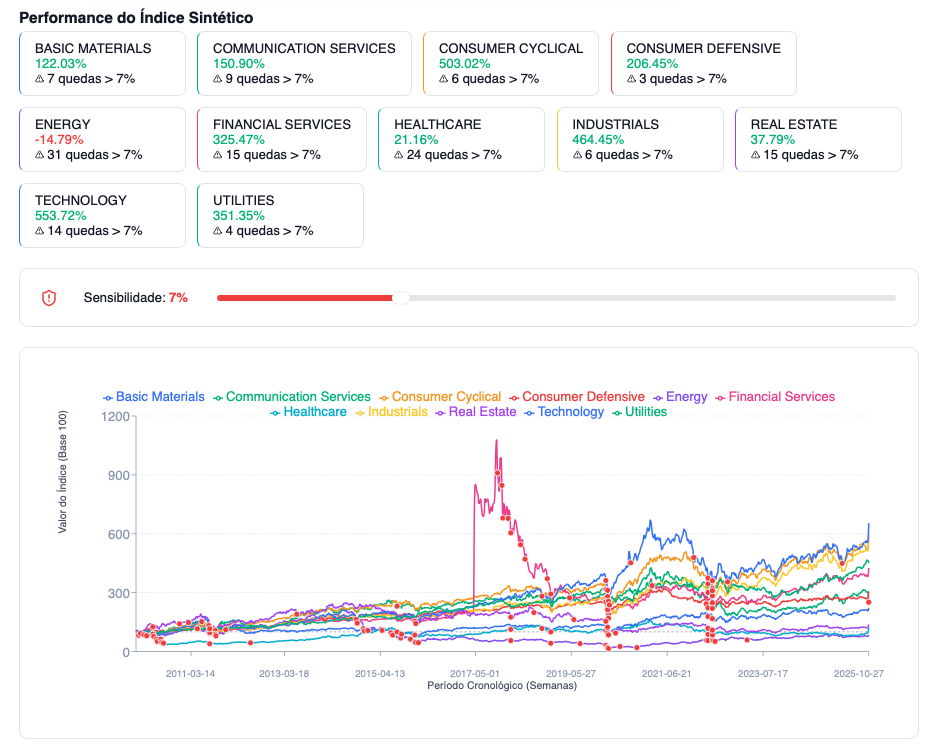
\includegraphics[width=\textwidth]{figuras/PerformanceIndiceSintetico1.png}
   \label{fig:performance-2010-2025}
   \fonte{Elaborado pelos autores.}
\end{figure}

A Figura~\ref{fig:performance-2010-2016} exibe o recorte da primeira metade da janela de análise, período no qual a maioria dos setores exibiu trajetória ascendente, com destaque para \textit{Consumer Cyclical} ($+161{,}69\%$), \textit{Communication Services} ($+147{,}11\%$), \textit{Utilities} ($+117{,}29\%$) e \textit{Technology} ($+111{,}26\%$). Dois casos contrariam a tendência geral do intervalo. O setor de \textit{Energy} encerrou o recorte com retorno acumulado de $-27{,}43\%$  e acumulou dezessete quedas semanais superiores a 7\%, comportamento consistente com o ciclo de queda dos preços internacionais do petróleo iniciado em meados de 2014, no qual o barril de Brent (referência global para preço de petróleo) recuou de aproximadamente 112 dólares em junho de 2014 para pouco mais de 30 dólares em janeiro de 2016, uma das maiores quedas de preço da \textit{commodity} registradas na história moderna ~\cite{baffes2015} e~\cite{baumeisterkilian2016}. O setor de \textit{Healthcare}, por sua vez, apresentou dezesseis quedas críticas e retorno negativo de $-20{,}79\%$, resultado que se alinha à volatilidade estrutural do subsetor de biotecnologia, cujas ações são sensíveis a resultados de ensaios clínicos e a decisões regulatórias da FDA (agência federal do governo dos Estados Unidos responsável por proteger a saúde pública), apresentando oscilações percentuais superiores às demais indústrias do setor~\cite{thakor2017,goleconvernon2009}.

\begin{figure}[htb]
   \centering
   \caption{Índice sintético setorial em base 100, período 2010 a 2016, sensibilidade de 7\%.}
   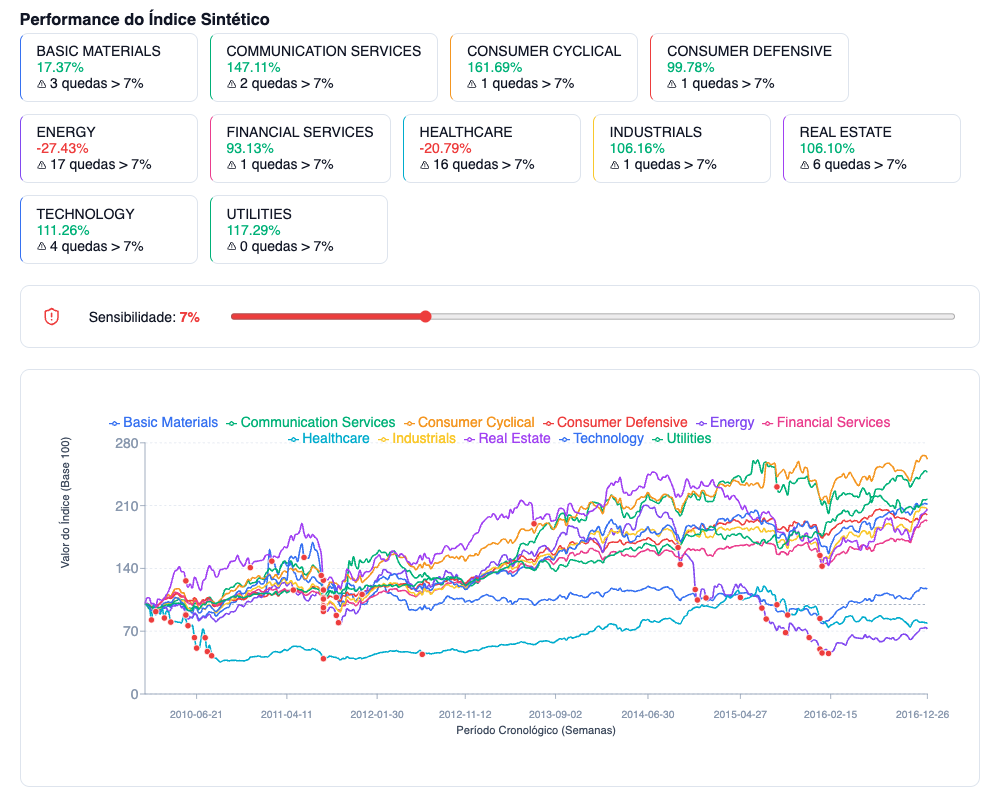
\includegraphics[width=\textwidth]{figuras/PerformanceIndiceSintetico4.png}
   \label{fig:performance-2010-2016}
   \fonte{Elaborado pelos autores.}
\end{figure}

A Figura~\ref{fig:performance-2016-2022} apresenta o recorte seguinte, no qual o efeito da pandemia de 2020 fica evidente pela concentração de quedas críticas em torno de março de 2020. Observa-se também um salto atípico na série do setor de \textit{Financial Services} entre 2017 e 2018, com o índice ultrapassando o valor 600. O comportamento decorre da entrada, no ano de 2017, de uma ação listada no mercado americano cotada a aproximadamente 48 mil dólares por unidade. Como o índice sintético do painel é equiponderado por ativo, a inclusão de um papel de preço tão elevado desloca a média setorial de forma abrupta, produzindo o degrau observado na trajetória de \textit{Financial Services}. A permanência dessa distorção evidencia a sensibilidade do índice equiponderado a ativos de preço absoluto extremo e reaparece nos painéis de Volatilidade e Sazonalidade, sendo retomada nas subseções correspondentes.

\begin{figure}[htb]
   \centering
   \caption{Índice sintético setorial em base 100, período 2016 a 2022, sensibilidade de 7\%.}
   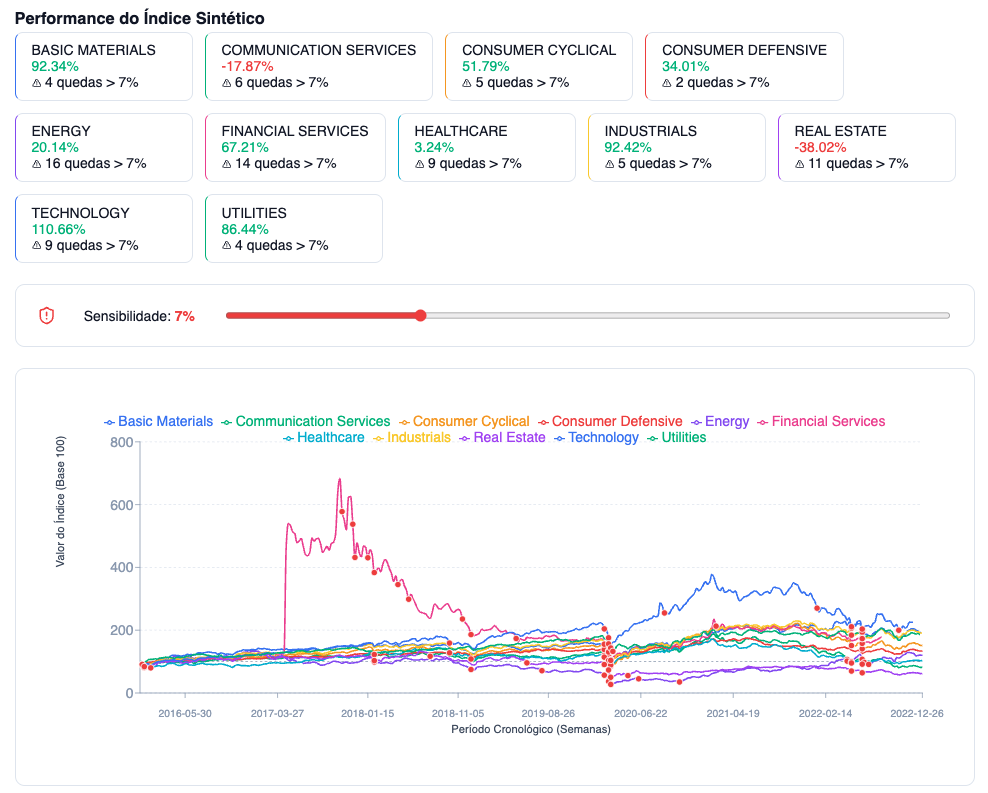
\includegraphics[width=\textwidth]{figuras/PerformanceIndiceSintetico2.png}
   \label{fig:performance-2016-2022}
   \fonte{Elaborado pelos autores.}
\end{figure}

A Figura~\ref{fig:performance-tech-re-hc} ilustra o uso da funcionalidade de filtragem por setor combinada com o ajuste do limiar de sensibilidade para 5\%. O recorte contrapõe três setores de comportamento distinto no período pós-pandêmico: \textit{Technology}, que acumulou retorno de $+110{,}66\%$ com pico próximo ao índice 380 no início de 2021; \textit{Real Estate}, que registrou $-38{,}02\%$ ao longo do intervalo, refletindo o ciclo de alta de juros; e \textit{Healthcare}, cujo retorno praticamente nulo ($+3{,}24\%$) esconde uma trajetória de recuperação após a queda pandêmica seguida de correção nos anos posteriores. A capacidade de isolar setores dessa forma é o que viabiliza a análise comparativa detalhada exigida pela metodologia de validação cruzada, retomada na Seção~\ref{sec:tabela-alocacao}.

\begin{figure}[htb]
   \centering
   \caption{Comparação setorial filtrada entre \textit{Technology}, \textit{Real Estate} e \textit{Healthcare}, período 2016 a 2022.}
   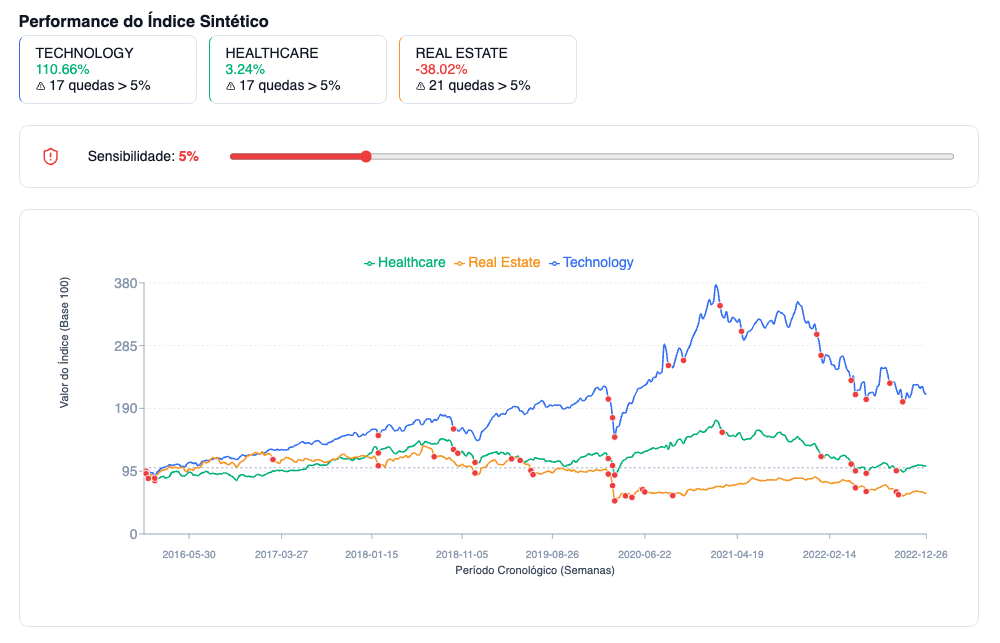
\includegraphics[width=\textwidth]{figuras/PerformanceIndiceSintetico3.png}
   \label{fig:performance-tech-re-hc}
   \fonte{Elaborado pelos autores.}
\end{figure}

\subsection{Painel de Volatilidade}
\label{subsec:painel-volatilidade}

O painel de Volatilidade expõe o desvio padrão anualizado dos retornos setoriais, permitindo comparar o risco total agregado por setor ao longo de diferentes janelas temporais. Percebe-se que a hierarquia de risco setorial não é constante ao longo dos anos: setores associados a alta volatilidade, como \textit{Energy}, mantêm posições elevadas na maior parte dos períodos, enquanto \textit{Utilities} e \textit{Consumer Defensive} figuram consistentemente entre os menos voláteis. A média de longo prazo, entretanto, suaviza episódios pontuais de volatilidade extrema que só ficam visíveis quando a série histórica completa é segmentada.

A Figura~\ref{fig:vol-2010-2016} apresenta o recorte inicial, no qual \textit{Healthcare} aparece como o setor mais volátil ($\approx 32\%$), seguido por \textit{Energy} ($\approx 30\%$). O resultado do setor de \textit{Healthcare} é coerente com a concentração de empresas de biotecnologia de menor porte na amostra, cujos preços respondem de forma acentuada a eventos regulatórios e resultados de ensaios clínicos.

\begin{figure}[htb]
   \centering
   \caption{Desvio padrão anualizado por setor, período 2010 a 2016.}
   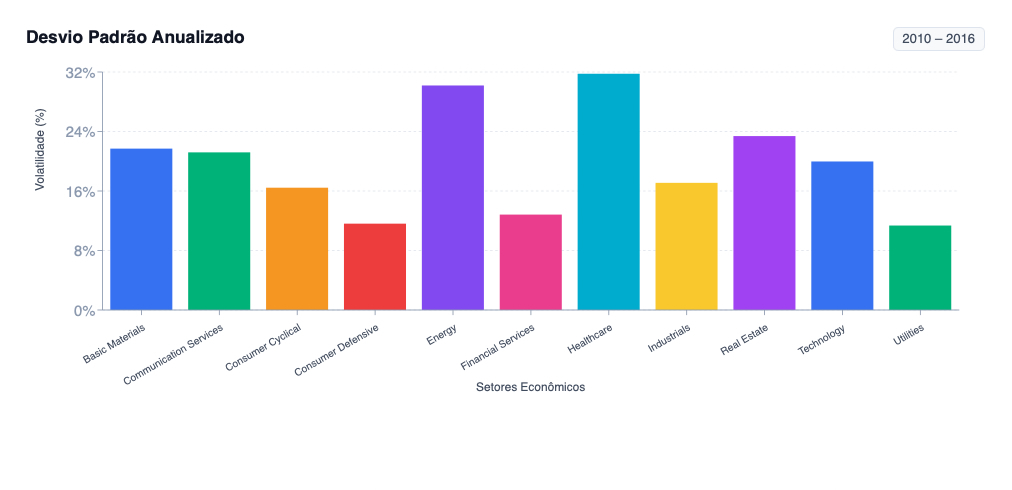
\includegraphics[width=\textwidth]{figuras/desviopadrao1016.jpg}
   \label{fig:vol-2010-2016}
   \fonte{Elaborado pelos autores.}
\end{figure}

A Figura~\ref{fig:vol-2016-2022} apresenta o recorte seguinte, no qual a barra do setor \textit{Financial Services} alcança patamar próximo a 108\%, valor destoante em relação aos demais setores. O fenômeno é a contraparte, no espaço de volatilidade, do mesmo evento discutido no painel de Performance: a entrada em 2017 de uma ação cotada a aproximadamente 48 mil dólares produziu um salto de nível na série do setor, e esse degrau, ao ser incorporado ao cálculo dos log-retornos usados na volatilidade anualizada, gera uma variação percentual pontual de magnitude muito superior às oscilações usuais, elevando artificialmente o desvio padrão do intervalo.

\begin{figure}[htb]
   \centering
   \caption{Desvio padrão anualizado por setor, período 2016 a 2022.}
   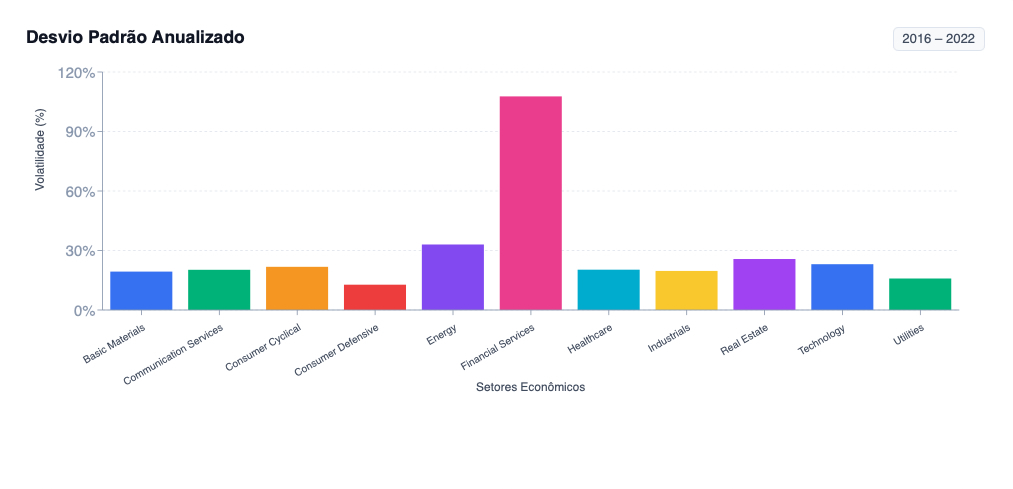
\includegraphics[width=\textwidth]{figuras/desviopadrao1622.jpg}
   \label{fig:vol-2016-2022}
   \fonte{Elaborado pelos autores.}
\end{figure}

A Figura~\ref{fig:vol-2020-2025} apresenta o recorte mais recente, no qual 
\textit{Energy} figura como o setor mais volátil ($\approx 33\%$), seguido por 
\textit{Technology} e \textit{Real Estate}, enquanto \textit{Utilities} e \textit{Consumer Defensive} ocupam 
a extremidade inferior. A hierarquia observada é coerente com o 
comportamento setorial já identificado no painel de Performance. A convergência dos setores em uma faixa mais estreita ($17\%$ a $33\%$) sugere que o período recente foi marcado 
por um regime de volatilidade mais uniforme entre setores, em contraste 
com a maior dispersão observada nos recortes anteriores.

\begin{figure}[htb]
   \centering
   \caption{Desvio padrão anualizado por setor, período 2020 a 2025.}
   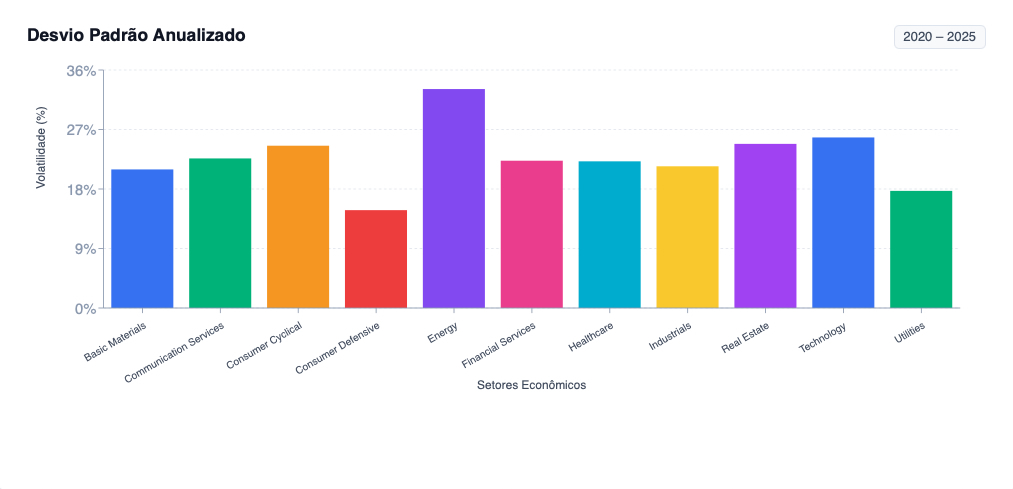
\includegraphics[width=\textwidth]{figuras/desviopadrao2025.jpg}
   \label{fig:vol-2020-2025}
   \fonte{Elaborado pelos autores.}
\end{figure}

\subsection{Painel de Sazonalidade}
\label{subsec:painel-sazonalidade}

O painel de Sazonalidade agrega o retorno médio mensal de cada setor ao longo da análise, permitindo identificar padrões anuais. A Figura~\ref{fig:sazonalidade-completa} apresenta a visão consolidada de 2010 a 2025, na qual se destaca um pico isolado no mês de abril para o setor de Financial Services, com retorno médio próximo a 3,8\%. O valor decorre da mesma anomalia já identificada nos painéis anteriores.

\begin{figure}[htb]
   \centering
   \caption{Retorno médio mensal por setor, período 2010 a 2025, visão completa.}
   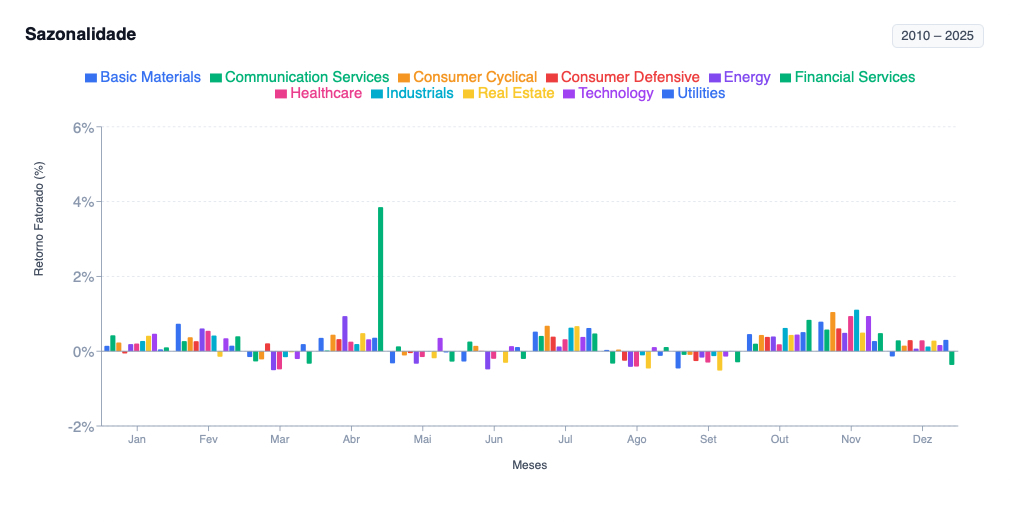
\includegraphics[width=\textwidth]{figuras/sazonalidadegeral.jpg}
   \label{fig:sazonalidade-completa}
   \fonte{Elaborado pelos autores.}
\end{figure}

Ao remover o setor afetado pelo filtro em cascata, obtém-se a Figura~\ref{fig:sazonalidade-filtrada}, na qual o padrão sazonal emerge com clareza. Observa-se retornos médios negativos ou próximos de zero entre agosto e setembro, seguidos por retornos positivos consistentes em outubro e novembro, com valores próximos a 1\% em vários setores. O padrão é aderente ao efeito sazonal documentado na literatura como \textit{Halloween Indicator} ou \textit{Sell in May}, segundo o qual o desempenho do mercado tende a ser mais fraco entre maio e outubro e mais forte entre novembro e abril, fenômeno originalmente identificado por~\citeonline{boumanjacobsen2002} e cuja persistência em amostras posteriores é discutida por~\citeonline{andrade2013}.

\begin{figure}[htb]
   \centering
   \caption{Retorno médio mensal por setor, período 2010 a 2025, visão completa.}
   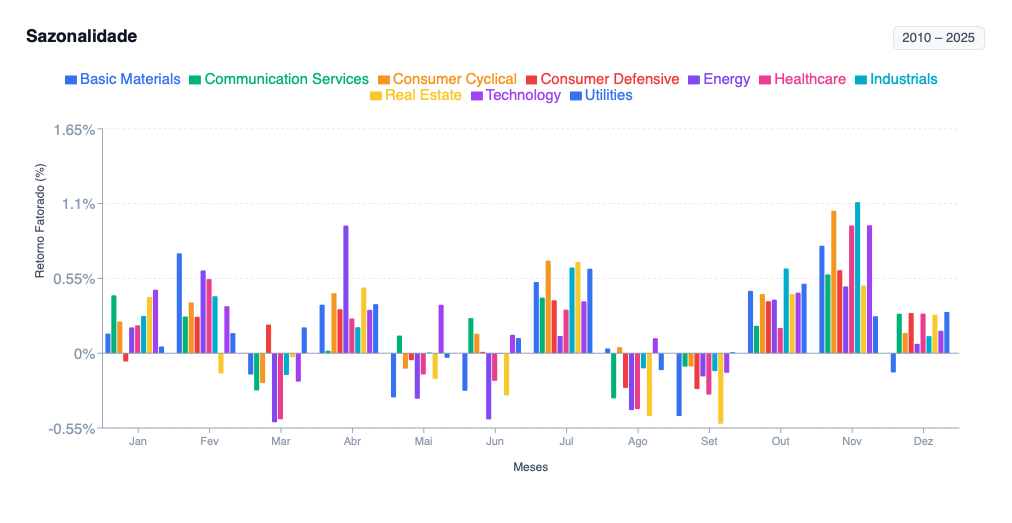
\includegraphics[width=\textwidth]{figuras/sazonalidadesemfs.jpg}
   \label{fig:sazonalidade-filtrada}
   \fonte{Elaborado pelos autores.}
\end{figure}

\subsection{Painel de Correlação}
\label{subsec:painel-correlacao}

O painel de Correlação apresenta a matriz de correlação de Pearson entre as séries semanais dos índices sintéticos setoriais, permitindo identificar setores que se movem em conjunto e setores que atuam como diversificadores. A Figura~\ref{fig:correlacao-setorial} exibe o resultado obtido para a série histórica completa de 2010 a 2025, oferecendo uma leitura das relações setoriais de longo prazo.

\begin{figure}[htb]
   \centering
   \caption{Matriz de correlação setorial calculada sobre séries semanais dos índices sintéticos, período 2010 a 2025.}
   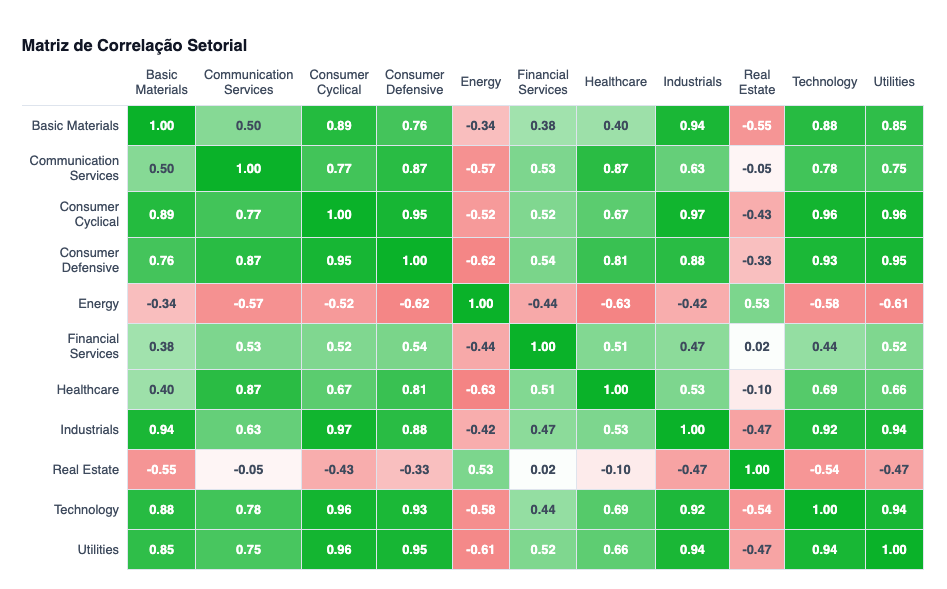
\includegraphics[width=\textwidth]{figuras/matriz.png}
   \label{fig:correlacao-setorial}
   \fonte{Elaborado pelos autores.}
\end{figure}

O bloco central da matriz revela correlações elevadas entre os setores, com valores próximos ou superiores a 0,90 entre \textit{Consumer Cyclical, Industrials, Technology, Utilities} e \textit{Consumer Defensive}. Esses setores tendem a acompanhar de forma conjunta o ciclo econômico, o que reduz sua efetividade como pares de diversificação dentro de uma carteira.

Dois setores destoam do padrão. \textit{Energy} apresenta correlações negativas com praticamente todos os demais, variando de $-0{,}34$ com \textit{Basic Materials} a $-0{,}63$ com \textit{Healthcare}, comportamento coerente com o papel do setor como reserva de valor em cenários inflacionários. \textit{Real Estate} exibe correlações negativas ou próximas de zero com a maioria dos setores, resultado influenciado pelo ciclo específico do setor imobiliário no período pós-2020, marcado pela alta de juros. A correlação positiva entre \textit{Energy} e \textit{Real Estate} ($+0{,}53$) sugere que ambos os setores compartilharam um mesmo regime de resposta a fatores macroeconômicos diferente dos outros setores.

\textit{Financial Services} aparece com correlações moderadas em relação aos demais setores, na faixa entre $0{,}38$ e $0{,}54$. Esse resultado é parcialmente influenciado pela anomalia de 2017 já discutida, cujo salto de nível na série do setor introduz um componente de variação não correlacionado com o comportamento macroeconômico dos demais setores, reduzindo os coeficientes calculados.

Essas observações têm implicação direta na construção de carteiras: a exposição simultânea a \textit{Energy} ou \textit{Real Estate} oferece potencial de diversificação superior ao observado dentro do bloco cíclico, informação que é incorporada de forma implícita no modelo de alocação discutido na Seção~\ref{sec:tabela-alocacao}.

\section{Análise de Risco}
\label{sec:evolucao-risco}

Concluída a análise dos conjuntos de ação por setor, o passo seguinte é observar como as ações se comportam ao longo do tempo quando agrupadas segundo a coluna \texttt{faixa\_risco}, materializada durante o ETL a partir dos cortes simétricos do \textit{Z-score} aplicados sobre \texttt{risco\_base}. As cinco faixas resultantes (Muito Baixo, Baixo, Médio, Alto e Muito Alto) formam portfólios equiponderados cuja trajetória histórica pode ser confrontada com o índice S\&P~500.

\subsection{Retorno Anualizado por Faixa de Risco}
\label{subsec:retorno-por-faixa}

A primeira visualização apura a média do retorno anualizado observado em cada portfólio agrupado por faixa de risco. Cada barra representa a rentabilidade anual composta da carteira formada pelas ações classificadas naquela faixa, apurada sobre o intervalo temporal indicado no cabeçalho do gráfico. A barra correspondente ao S\&P~500 fornece a referência de mercado calculada sobre a mesma janela.

A Figura~\ref{fig:retorno-faixa-full} exibe o retorno médio do período completo de análise, de 2010 a 2025.

\begin{figure}[htb]
   \centering
   \caption{Retorno anualizado por faixa de risco no período de 2010 a 2025.}
   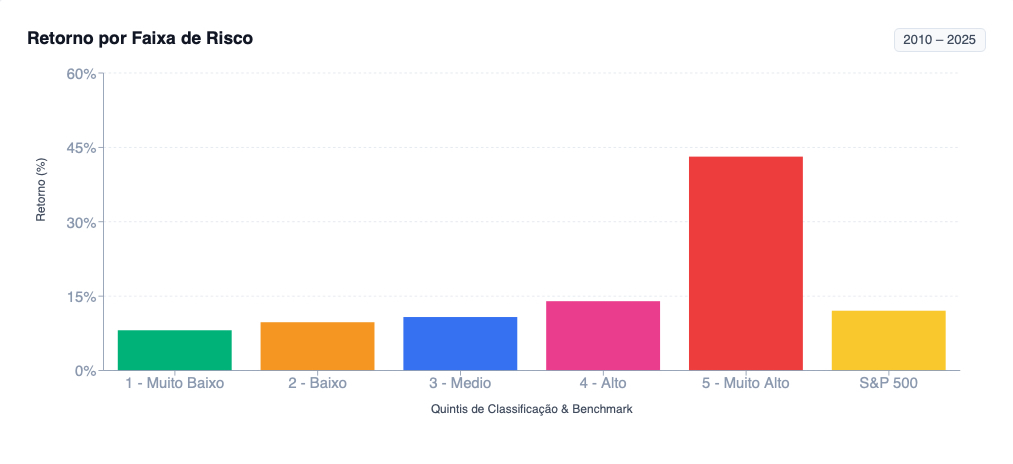
\includegraphics[width=0.85\textwidth]{figuras/Retornogeral.jpg}
   \label{fig:retorno-faixa-full}
   \fonte{Elaborado pelos autores.}
\end{figure}

Ao longo do período dado, os retornos das quatro faixas de menor risco e do próprio S\&P~500 concentram-se entre 8\% e 14\% ao ano, com pequena separação entre elas. A faixa Muito Alto isola-se acima de 40\% anualizados. A leitura desses valores demanda, contudo, uma qualificação metodológica: a métrica apresentada corresponde à média aritmética dos retornos semanais das ações agrupadas em cada faixa, anualizada por multiplicação simples. Esse procedimento tende a superestimar o retorno composto efetivo em séries de alta volatilidade, uma vez que a média aritmética supera a média geométrica na presença de dispersão dos retornos. Como a faixa Muito Alto concentra os ativos de maior variabilidade do universo, o valor agregado observado nesse painel deve ser interpretado como uma leitura descritiva do comportamento médio das ações que compõem a faixa, e não como o retorno efetivamente realizável por uma carteira equiponderada mantida ao longo do intervalo. 

O segundo recorte, na Figura~\ref{fig:retorno-faixa-calmo}, restringe a análise ao intervalo de 2012 a 2015, marcado por baixa volatilidade, e ausência de rupturas relevantes no mercado norte-americanos.

\begin{figure}[htb]
   \centering
   \caption{Retorno anualizado por faixa de risco no período de 2012 a 2015.}
   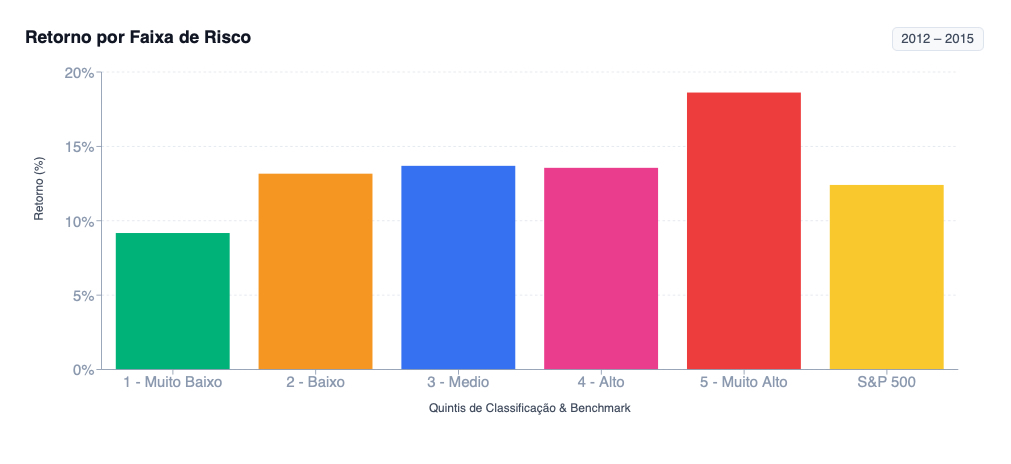
\includegraphics[width=0.85\textwidth]{figuras/retorno1215.jpg}
   \label{fig:retorno-faixa-calmo}
   \fonte{Elaborado pelos autores.}
\end{figure}
  
Sob esse recorte, a hierarquia entre faixas se comprime consideravelmente, com e a diferença entre a faixa Muito Alto e a faixa Muito Baixo reduz-se a cerca de 10 pontos percentuais. O S\&P~500 posiciona-se no interior da distribuição, próximo à faixa Médio. O quadro sugere que o prêmio associado às faixas de risco mais elevadas exige um tempo suficientemente longo para se materializar. 

O terceiro recorte, apresentado na Figura~\ref{fig:retorno-faixa-covid}, cobre o intervalo de 2020 a 2023, período que engloba o choque pandêmico e a recuperação subsequente dos mercados.

\begin{figure}[htb]
   \centering
   \caption{Retorno anualizado por faixa de risco no período de 2020 a 2023.}
   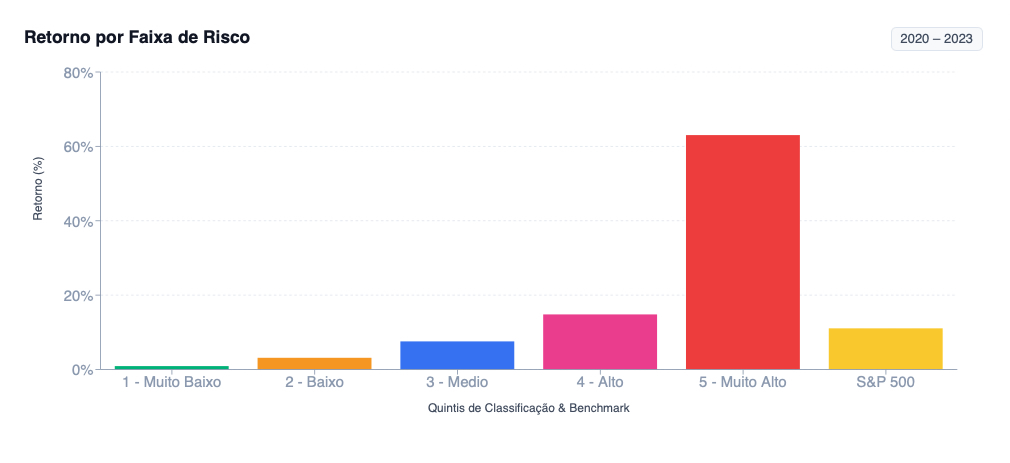
\includegraphics[width=0.85\textwidth]{figuras/retorno2023.jpg}
   \label{fig:retorno-faixa-covid}
   \fonte{Elaborado pelos autores.}
\end{figure}

O comportamento inverte-se em intensidade em relação à janela calma. A faixa Muito Alto ultrapassa 60\% na métrica agregada, enquanto as faixas Muito Baixo e Baixo permanecem próximas de zero, e o S\&P~500 mantém-se em torno de 11\%. A amplificação observada é coerente com a definição do Beta \cite{sharpe1964}, segundo a qual ativos de maior sensibilidade ao mercado apresentam movimentos direcionais amplificados; a metodologia adotada intensifica esse efeito em janelas de alta dispersão dos retornos, o que reforça o contraste visual entre a faixa de risco elevado e as demais.


O conjunto das três janelas evidencia que a métrica composta responde de forma coerente ao regime macroeconômico observado. Em longos períodos, o valor agregado sugere uma hierarquia entre faixas; em janelas curtas de tranquilidade, essa hierarquia se achata e o critério perde poder discriminante; em janelas dominadas por choque e recuperação, os valores se acentuam. Essa sensibilidade ao regime evidencia que a métrica captura características de risco suficientemente informativas para separar comportamentos distintos em diferentes contextos macroeconômicos, o que sustenta a apresentação dos recortes seguintes desta seção.

\subsection{Retração Máxima por Faixa de Risco}
\label{subsec:mdd}

O segundo painel analisa a intensidade das perdas extremas experimentadas por cada portfólio ao longo do intervalo selecionado. A métrica utilizada é o \textit{maximum drawdown} (MDD), que mede a maior retração percentual observada entre um pico e o vale subsequente da série de valor da carteira. Enquanto o retorno anualizado reflete o resultado médio composto, o MDD captura a exposição a perdas extremas, dimensão essencial para caracterizar o risco enfrentado pelo investidor durante o percurso.

\begin{figure}[htb]
   \centering
   \caption{\textit{Maximum drawdown} por faixa de risco no período de 2010 a 2025.}
   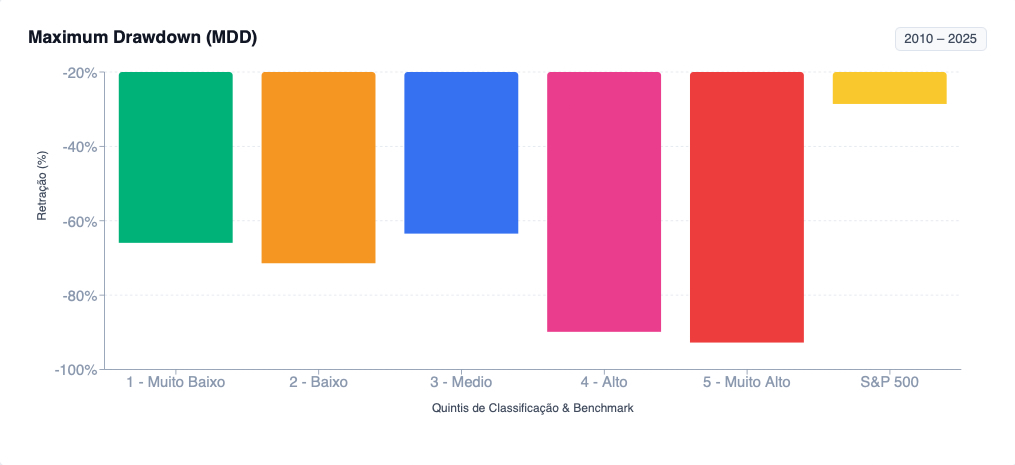
\includegraphics[width=0.85\textwidth]{figuras/mddgeral.jpg}
   \label{fig:mdd-full}
   \fonte{Elaborado pelos autores.}
\end{figure}

A Figura~\ref{fig:mdd-full} exibe o MDD apurado para o período completo de 2010 a 2025. A leitura do gráfico identifica dois grupos distintos. As três faixas de menor risco (Muito Baixo, Baixo e Médio) apresentam retrações máximas entre 63\% e 72\%, com pouca variação entre si. As duas faixas de risco mais elevado (Alto e Muito Alto) exibem MDD de aproximadamente 90\% e 93\%, respectivamente. A distância entre os dois grupos, próxima de 20 pontos percentuais, evidencia que o critério proposto separa efetivamente ativos com tolerância distinta a quedas extremas. O S\&P~500 registra MDD de aproximadamente 25\% na mesma janela, valor substancialmente inferior ao apurado em qualquer faixa individual. A diferença reflete o efeito da diversificação ampla do índice frente às carteiras equiponderadas por faixa, que operam sobre subconjuntos mais restritos do universo.

A Figura~\ref{fig:mdd-pre-pandemia} apresenta o mesmo painel para o intervalo de 2010 a 2017, período anterior à pandemia.

\begin{figure}[htb]
   \centering
   \caption{\textit{Maximum drawdown} por faixa de risco no período de 2010 a 2017.}
   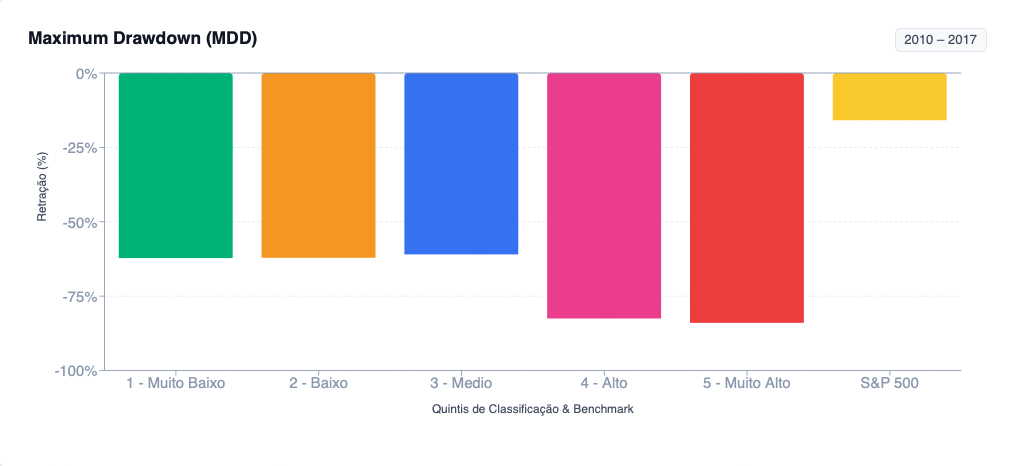
\includegraphics[width=0.85\textwidth]{figuras/mdd1017.jpg}
   \label{fig:mdd-pre-pandemia}
   \fonte{Elaborado pelos autores.}
\end{figure}

Neste recorte, a separação entre os dois grupos torna-se ainda mais nítida. As faixas Muito Baixo, Baixo e Médio concentram-se em retrações próximas de 60\%, enquanto Alto e Muito Alto atingem 83\% e 85\%. O S\&P~500 registra MDD de aproximadamente 15\%, valor coerente com a característica de menor turbulência desse intervalo. 

A Figura~\ref{fig:mdd-pandemia} restringe a análise ao intervalo de 2019 a 2023.

\begin{figure}[htb]
   \centering
   \caption{\textit{Maximum drawdown} por faixa de risco no período de 2019 a 2023.}
   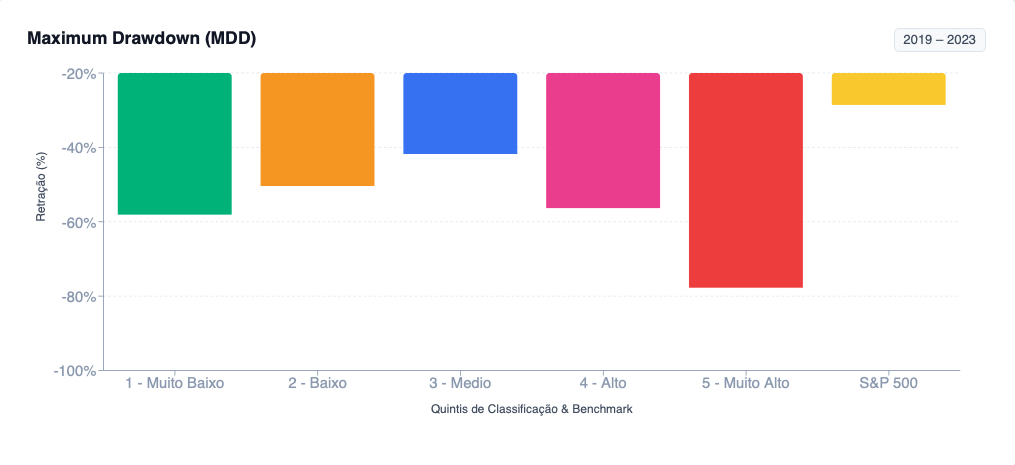
\includegraphics[width=0.85\textwidth]{figuras/mdd1923.jpg}
   \label{fig:mdd-pandemia}
   \fonte{Elaborado pelos autores.}
\end{figure}

Sob o recorte pandêmico, a ordenação por faixa perde regularidade. A faixa Médio registra a menor retração entre as carteiras, próximo de 42\%, seguida por Baixo com 50\%, Alto com 56\% e Muito Baixo com 58\%. Apenas a faixa Muito Alto isola-se claramente do restante, com MDD de aproximadamente 77\%. O S\&P~500 apresenta retração de cerca de 27\%. O padrão indica que, em janelas curtas dominadas por um choque agudo, a hierarquia entre faixas intermediárias se dissolve: o evento afeta simultaneamente carteiras de perfis distintos, deslocando a leitura do risco relativo. Apenas a faixa Muito Alto preserva separação inequívoca em relação ao restante do universo, o que confirma sua identificação consistente como zona de risco elevado independentemente do regime da janela.

O conjunto dos três recortes sustenta que a métrica proposta discrimina de forma robusta os extremos da escala de risco em termos de perda máxima. A distância entre a faixa Muito Alto e as demais é preservada em todos os intervalos analisados. A discriminação dentro do grupo de menor risco é menos estável e sensível ao regime da janela, particularmente quando um evento sistêmico afeta o mercado como um todo.

\subsection{Exposição Setorial de Risco}
\label{subsec:exposicao-setorial}

O terceiro painel desloca a granularidade da análise do nível de faixa individual para o nível setorial. A visualização apresenta o Z-score médio de \texttt{risco\_base} agregado por setor econômico, calculado sobre a janela selecionada. Setores com Z-score positivo abrigam ações cujo risco médio se encontra acima da média do universo, enquanto setores com Z-score negativo concentram ações de risco inferior à média. A leitura desse painel contextualiza os resultados agregados apresentados anteriormente ao indicar de quais segmentos do mercado provêm as ações classificadas em cada faixa.

\begin{figure}[htb]
   \centering
   \caption{\textit{Z-score} médio de risco por setor no período de 2010 a 2025.}
   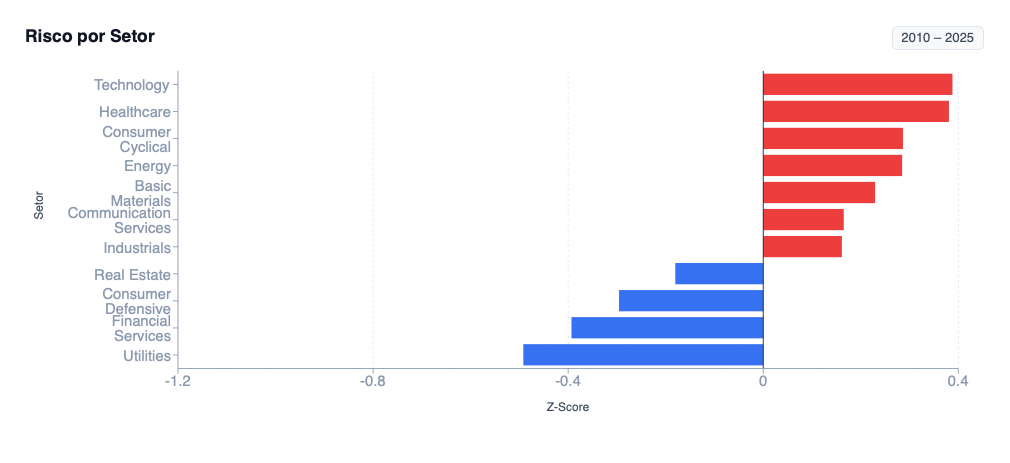
\includegraphics[width=0.85\textwidth]{figuras/riscopsgeral.jpg}
   \label{fig:risco-setor-full}
   \fonte{Elaborado pelos autores.}
\end{figure}

A Figura~\ref{fig:risco-setor-full} apresenta o quadro consolidado para o período de 2010 a 2025. A parte superior do gráfico é ocupada por \textit{Technology e Healthcare}, ambos com Z-score próximo de 0{,}4, seguidos de \textit{Consumer Cyclical} e \textit{Energy}, com aproximadamente 0{,}3, e por \textit{Basic Materials, Communication Services e Industrials} em posições intermediárias entre 0{,}1 e 0{,}2. Na região negativa, Utilities destaca-se como o setor de menor risco, com Z-score próximo de $-0{,}5$, seguido por Financial \textit{Services, Consumer Defensive} e \textit{Real Estate}. A ordenação obtida é coerente com a caracterização usual de setores sensíveis à atividade econômica: os primeiros ocupam a região positiva do gráfico, os segundos, a região negativa. O painel confirma que o critério de risco desenvolvido reproduz distinções setoriais compatíveis com a intuição de mercado quando aplicado sobre um período amplo.

\begin{figure}[htb]
   \centering
   \caption{\textit{Z-score} médio de risco por setor no período de 2019 a 2023.}
   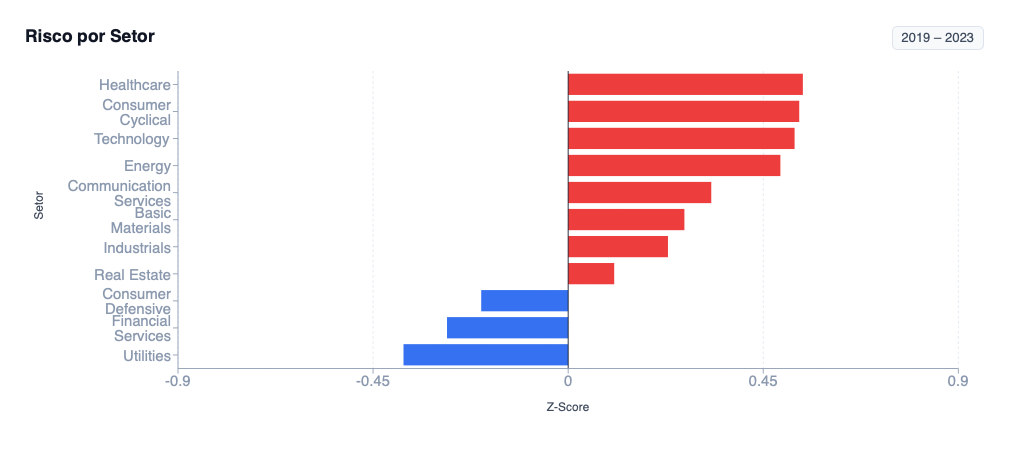
\includegraphics[width=0.85\textwidth]{figuras/riscops1923.jpg}
   \label{fig:risco-setor-pandemia}
   \fonte{Elaborado pelos autores.}
\end{figure}

A Figura~\ref{fig:risco-setor-pandemia} restringe a análise ao intervalo de 2019 a 2023. Dois deslocamentos merecem destaque neste recorte. O primeiro é a subida geral de magnitude entre os setores da região positiva: \textit{Healthcare, Consumer Cyclical e Technology} agrupam-se próximos de 0{,}5 desvio padrão acima da média, valores superiores aos observados no painel consolidado. A concentração indica que o intervalo pandêmico ampliou de forma sincronizada o risco associado aos setores sensíveis à variação de atividade econômica e aos setores de crescimento, resultado consistente com o choque de 2020 e a fase de reprecificação subsequente. O segundo deslocamento é a migração de \textit{Real Estate}, que abandona a região negativa e passa a apresentar Z-score levemente positivo. O comportamento é compatível com o impacto direto da pandemia sobre imóveis comerciais e a instabilidade subsequente do setor.

A comparação dos dois recortes demonstra que o painel de exposição setorial responde de forma sensível ao regime de cada janela. Os setores preservam sua natureza fundamental (defensiva ou sensível à atividade econômica) na ordenação geral, mas a intensidade relativa do risco entre eles varia conforme os choques específicos do intervalo. Essa sensibilidade sustenta o uso do painel como instrumento de contextualização: quando um setor específico é impactado por um evento macroeconômico, sua contribuição para as carteiras equiponderadas por faixa se altera, o que se propaga para as métricas agregadas apresentadas nas subseções anteriores.

\section{Análise de Alocação}
\label{sec:consultas-alocacao}

Esta seção reúne os painéis do \textit{dashboard} que tratam da lógica de alocação de capital. É também nesta seção que a validação cruzada contra o S\&P 500 é discutida em detalhe, especialmente na análise dos testes de alocação, que confrontam o desempenho da carteira construída a partir dos critérios de risco e fundamentos com o desempenho do índice de referência.

A ordem de apresentação parte da alocação mais simples possível, na qual todos os ativos de uma mesma faixa recebem peso idêntico, para, em seguida, discutir a construção da carteira e, por fim, a evolução comparativa dessa carteira contra o \textit{benchmark}.

\subsection{Painel de Evolução por Risco}
\label{subsec:painel-evolucao-risco}

O painel de Evolução por Risco apresenta o desempenho temporal de cinco portfólios equiponderados, um para cada faixa de risco definida pelo modelo, comparados ao S\&P 500 em base 100. Trata-se, portanto, de uma leitura direta do desempenho médio das ações agrupadas por classe de risco, sem interferência da lógica de alocação discutida na Seção~\ref{sec:tabela-alocacao}.

\begin{figure}[htb]
   \centering
   \caption{Evolução temporal dos portfólios equiponderados por faixa de risco e S\&P 500, base 100, período 2010 a 2025.}
   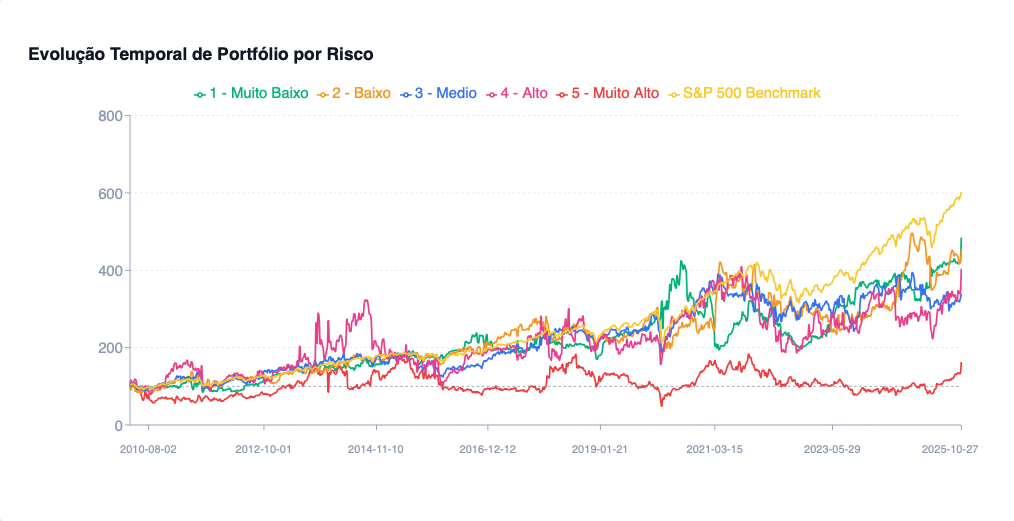
\includegraphics[width=\textwidth]{figuras/evolucaogeral.jpg}
   \label{fig:evolucao-risco-2010-2025}
   \fonte{Elaborado pelos autores.}
\end{figure}

A Figura~\ref{fig:evolucao-risco-2010-2025} apresenta o painel para o período completo de 2010 a 2025. O S\&P 500 encerra o período próximo do índice 600, superando todos os portfólios do modelo ao final da janela analisada. Os portfólios das faixas Muito Baixo, Baixo, Médio e Alto se agrupam em uma banda que oscila entre os índices 300 e 500 ao longo dos últimos anos da série, com trajetórias razoavelmente próximas entre si, ainda que apresentando volatilidades e picos distintos ao longo do tempo. A faixa Muito Alto, por sua vez, destoa negativamente do restante, permanecendo próxima ou abaixo do índice 100 durante boa parte do intervalo e encerrando o período em patamar inferior aos demais.

O desempenho insatisfatório da faixa Muito Alto é o achado mais marcante do painel. A leitura direta é a de que agrupar em um mesmo portfólio, com pesos iguais, todos os ativos classificados como de risco muito elevado gera um resultado agregado consistentemente pior que o das demais faixas ao longo do tempo, corroborando o \textit{paradoxo da baixa volatilidade} discutido na fundamentação teórica: ações de maior risco não entregam, em média, o retorno adicional que a hipótese clássica de risco e retorno prevê.

Uma ressalva importante para a interpretação é a natureza equiponderada da construção. Como todos os ativos recebem o mesmo peso dentro de cada faixa, sem qualquer critério de qualidade que diferencie empresas com fundamentos sólidos de empresas com fundamentos frágeis, a faixa Muito Alto absorve o efeito das ações mais deterioradas do conjunto analisado, que tendem a se concentrar nessa classificação. O painel, portanto, não apresenta um teste de estratégia de investimento propriamente dito, mas sim uma visualização do desempenho médio das faixas.

A distância entre os portfólios do modelo e o S\&P 500 ao final do período também merece atenção. Assim como observado nos painéis anteriores, o S\&P 500 opera sob ponderação por valor de mercado, o que atribui peso majoritário às maiores empresas do mercado americano. Os portfólios do modelo, ao equiponderarem centenas de ativos por faixa, diluem essa concentração e refletem um desempenho médio mais próximo do conjunto amplo de ações listadas na NYSE e na NASDAQ, cuja mediana de retorno é inferior à média ponderada por capitalização.

\subsection{Painel de Listagem de Ações}
\label{subsec:painel-listagem}

O painel de Listagem de Ações apresenta a granularidade máxima do \textit{dashboard}, exibindo o universo completo de ativos analisados em formato tabular, com uma linha por ação e colunas dedicadas às informações descritivas. A visualização funciona como a camada de detalhamento do ambiente analítico, complementando os painéis agregados apresentados até aqui: enquanto as análises setoriais e por faixa de risco oferecem leituras consolidadas, esta tabela permite descer ao ativo individual, inspecionando quais ações compõem cada agrupamento e como cada uma se posiciona segundo os critérios de risco desenvolvidos no trabalho.

\begin{figure}[htb]
   \centering
   \caption{Painel de Listagem de Ações com filtros de peso ativos para os modificadores de risco.}
   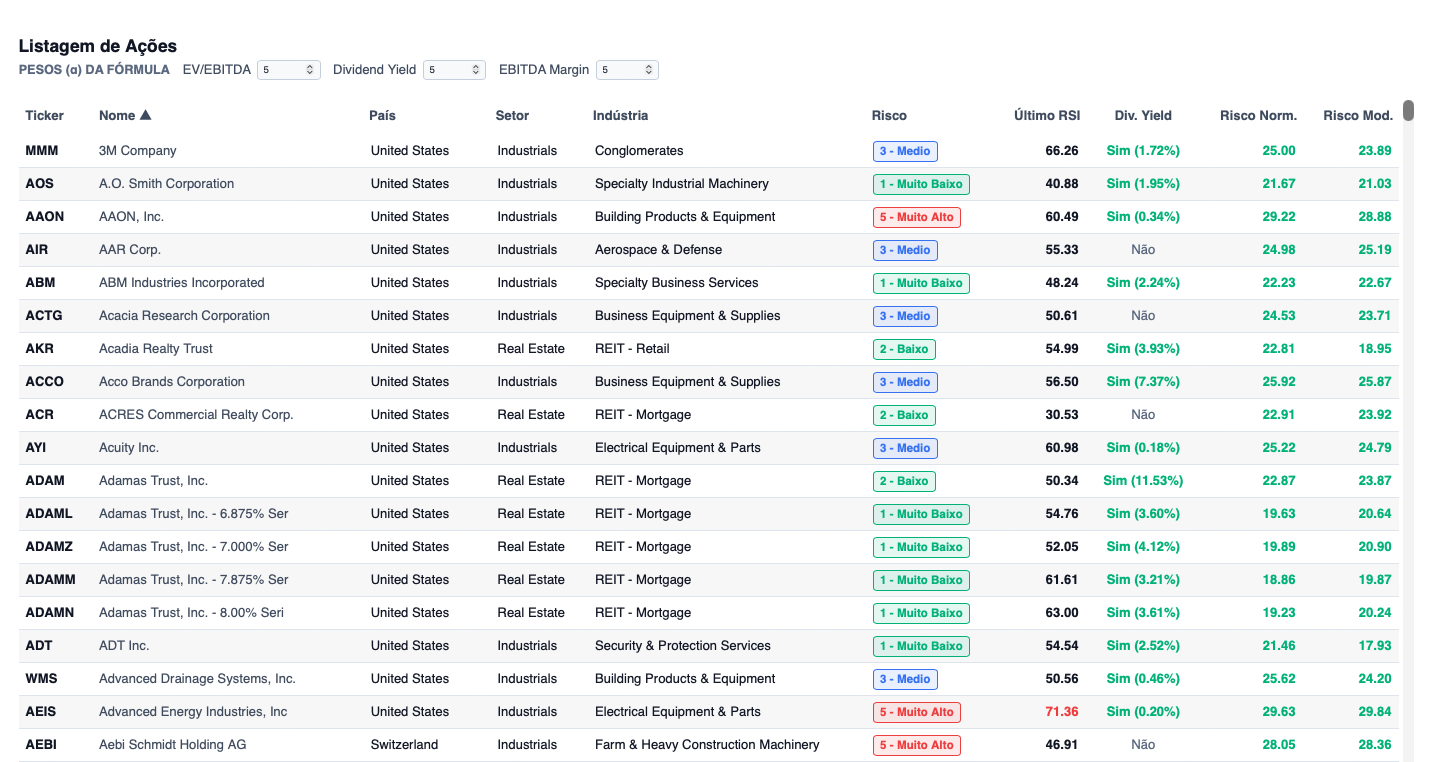
\includegraphics[width=\textwidth]{figuras/listagem.jpg}
   \label{fig:listagem-acoes}
   \fonte{Elaborado pelos autores.}
\end{figure}

A Figura~\ref{fig:listagem-acoes} apresenta a tela do painel. Cada linha reúne o \textit{ticker}, o nome da empresa, o país de listagem, o setor e a indústria de classificação, a faixa de risco atribuída pelo modelo, o \textit{Trailing RSI}, o \textit{Trailing Dividend Yield} indicado como sinalizador binário acompanhado do valor percentual, e as duas versões do risco calculado, o Risco Normalizado e o Risco Modificado. A tabela é ordenável por qualquer uma dessas colunas, permitindo ao usuário reorganizar a listagem pelas dimensões que julgar pertinentes à sua investigação.

O aspecto mais relevante do painel, entretanto, não é a exibição estática da tabela, mas a capacidade de intervenção do usuário sobre a fórmula do Risco Modificado. Os três seletores numéricos posicionados no topo da tela permitem ajustar os pesos $\alpha_{EV}$, $\alpha_{DY}$ e $\alpha_{EB}$ associados, respectivamente, aos modificadores EV/EBITDA, \textit{Trailing Dividend Yield} e Margem EBITDA. Zerando o peso de um modificador, sua contribuição desaparece da composição do risco, permitindo isolar o efeito individual de cada componente. Elevando o peso, sua influência relativa cresce linearmente, permitindo observar como a hierarquia de risco entre os ativos se reorganiza sob diferentes calibrações.

\subsection{Painel de Teste de Alocação e Validação Cruzada}
\label{sec:tabela-alocacao}

Esta subseção apresenta o resultado central do trabalho, no qual todos os componentes desenvolvidos ao longo do projeto operam em conjunto para produzir a validação cruzada da abordagem proposta contra o S\&P 500. A partir dos Testes de Alocação, o usuário seleciona um conjunto de ativos cuja combinação passa a compor um índice customizado, cujo desempenho histórico é reescalado em base 100 e confrontado diretamente com a série do índice de referência ao longo do intervalo de análise.

O experimento reportado adota um protocolo padronizado, replicado para cada uma das cinco faixas de risco. Para cada faixa, é selecionado o conjunto das dez ações com maior alocação percentual recomendada pelo modelo, sem aplicação dos modificadores de risco. Essa configuração permite avaliar o desempenho da lógica de seleção em sua forma mais direta, sem interferência das personalizações discutidas na subseção anterior, e produz um teste comparável entre as faixas.

\subsubsection{Faixa Muito Baixo}
\label{subsubsec:validacao-muito-baixo}

A Figura~\ref{fig:validacao-muito-baixo} apresenta o resultado do índice customizado composto pelas dez ações de maior alocação recomendada dentro da faixa Muito Baixo.

\begin{figure}[htb]
   \centering
   \caption{Desempenho histórico do índice customizado da faixa Muito Baixo contra o S\&P 500, base 100, período 2010 a 2025.}
   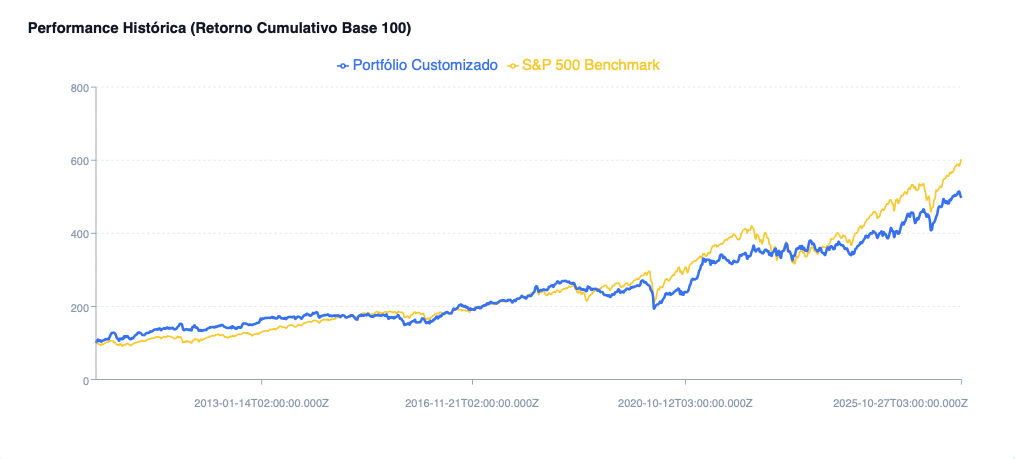
\includegraphics[width=\textwidth]{figuras/perfmuitobaixosem.jpg}
   \label{fig:validacao-muito-baixo}
   \fonte{Elaborado pelos autores.}
\end{figure}

O índice customizado da faixa Muito Baixo encerra o período próximo ao valor 500, contra aproximadamente 600 do S\&P 500 no mesmo marco temporal. A trajetória do portfólio construído pelo modelo acompanha a do \textit{benchmark}, com forte aderência visual entre as duas séries, especialmente no intervalo anterior a 2020. A partir de 2021, observa-se uma ampliação gradual da diferença entre as trajetórias, com o S\&P 500 assumindo desempenho progressivamente superior nos anos finais da série.

O resultado tem duas leituras complementares. Do ponto de vista da validação da abordagem, a proximidade entre as duas séries ao longo de quinze anos é o principal indicador de sucesso: um portfólio composto por apenas dez ações, selecionadas exclusivamente por critérios de risco e fundamentos e sem qualquer ajuste no tempo, replica de forma coerente o comportamento agregado do principal índice de referência do mercado americano. A aderência não decorre de sobreposição de ativos, uma vez que o S\&P 500 é ponderado por valor de mercado e concentra peso nas maiores capitalizações, enquanto o índice customizado seleciona empresas segundo o \textit{Z-Score} de qualidade da fórmula de risco, com ponderação exponencial sobre esse \textit{score}. A convergência entre as duas trajetórias, portanto, é um resultado emergente do modelo, e não um efeito de composição.

Do ponto de vista da discrepância residual, a distância ao final do período é coerente com o perfil defensivo da faixa selecionada. Ao restringir o universo a ativos classificados como de risco muito baixo, o modelo prioriza empresas com menor volatilidade e menor Beta, características que tendem a produzir retornos agregados inferiores em cenários de forte apreciação do mercado. O intervalo pós-2021, que incluiu ciclos de alta expressividade concentrados em grandes ativos de tecnologia com peso majoritário no S\&P 500, é exatamente o tipo de cenário no qual essa característica se torna mais visível. A distância observada, portanto, não indica falha do modelo, mas sim a consequência natural do compromisso entre proteção e retorno assumido ao se escolher a faixa mais defensiva do modelo como base do portfólio.

\subsubsection{Faixa Baixo}
\label{subsubsec:validacao-baixo}

A Figura~\ref{fig:validacao-baixo} apresenta o resultado do índice customizado composto pelas dez ações de maior alocação recomendada dentro da faixa Baixo.

\begin{figure}[htb]
   \centering
   \caption{Desempenho histórico do índice customizado da faixa Baixo contra o S\&P 500, base 100, período 2010 a 2025.}
   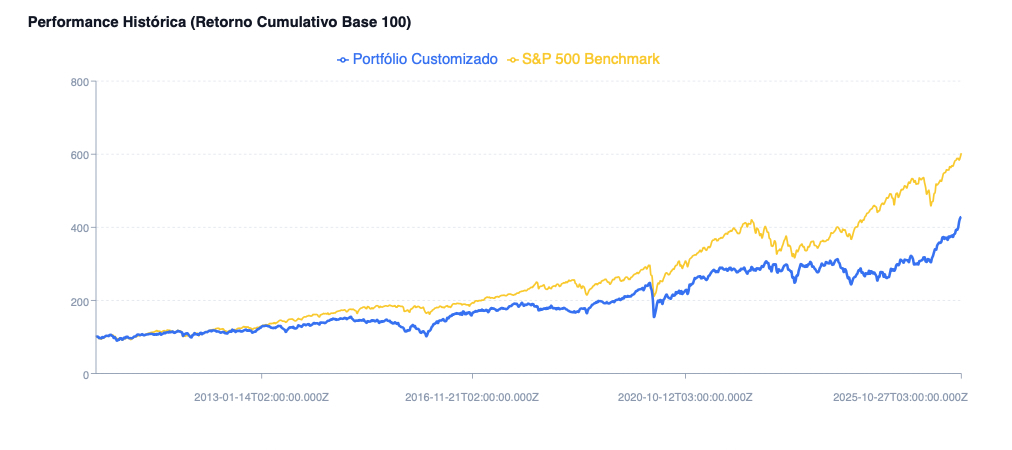
\includegraphics[width=\textwidth]{figuras/perfbaixosem.jpg}
   \label{fig:validacao-baixo}
   \fonte{Elaborado pelos autores.}
\end{figure}

O índice customizado da faixa Baixo encerra o período em torno do valor 430, contra aproximadamente 600 do S\&P 500 no mesmo marco temporal, produzindo uma diferença de desempenho superior à observada no portfólio da faixa Muito Baixo, discutida na Seção~\ref{subsubsec:validacao-muito-baixo}. A trajetória do portfólio acompanha o \textit{benchmark} ao longo da primeira metade do período, com boa aderência até aproximadamente 2016, mas a partir desse ponto o descolamento entre as duas séries se torna persistente, ampliando-se de forma praticamente contínua até o final do período.

O resultado é digno de nota por ser contraintuitivo à hipótese clássica de risco e retorno, segundo a qual portfólios de risco marginalmente maior deveriam entregar retornos agregados marginalmente superiores em intervalos longos. Aqui observa-se o oposto: o portfólio da faixa Baixo apresenta desempenho consistentemente inferior ao da faixa Muito Baixo, e a diferença não é episódica, mas se manifesta ao longo de praticamente todo o intervalo analisado. Esse comportamento é aderente ao \textit{paradoxo da baixa volatilidade} já mencionado na Seção~\ref{subsec:painel-evolucao-risco}, no qual ativos classificados como de menor risco tendem a entregar retornos ajustados iguais ou superiores aos de ativos de risco moderado, contrariando a expectativa derivada do modelo CAPM.

\subsubsection{Faixa Médio}
\label{subsubsec:validacao-medio}

A Figura~\ref{fig:validacao-medio-sem-mod} apresenta o resultado do índice customizado composto pelas dez ações de maior alocação recomendada dentro da faixa Médio.

\begin{figure}[htb]
   \centering
   \caption{Desempenho histórico do índice customizado da faixa Médio contra o S\&P 500, base 100, período 2010 a 2025, sem aplicação dos modificadores.}
   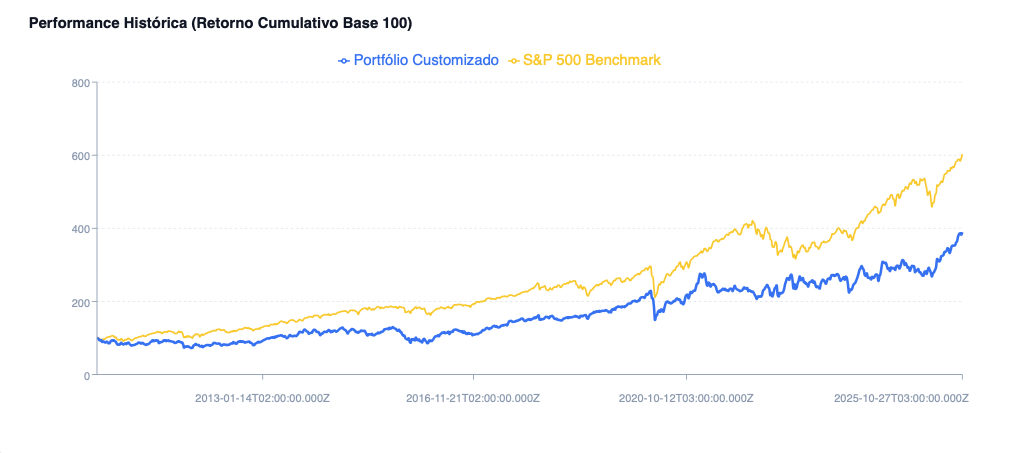
\includegraphics[width=\textwidth]{figuras/perfmediosem.jpg}
   \label{fig:validacao-medio-sem-mod}
   \fonte{Elaborado pelos autores.}
\end{figure}

O portfólio encerra o período próximo do valor 380, contra aproximadamente 600 do S\&P 500 no mesmo marco temporal, produzindo uma distância comparável à observada na faixa Baixo. A trajetória apresenta boa aderência ao \textit{benchmark} até por volta de 2018 e passa a descolar de forma mais visível nos anos finais da série, comportamento similar ao da faixa imediatamente anterior.

A Figura~\ref{fig:validacao-medio-com-mod} apresenta o mesmo experimento sob outra configuração, agora com a aplicação dos modificadores de risco previstos no modelo. Os pesos $\alpha_{EV}$, $\alpha_{DY}$ e $\alpha_{EB}$ foram ativados na fórmula do Risco Modificado, alterando o cálculo do risco individual de cada ativo e, por consequência, tanto a composição do top 10 de maior alocação recomendada quanto os pesos atribuídos a cada ação selecionada.

\begin{figure}[htb]
   \centering
   \caption{Desempenho histórico do índice customizado da faixa Médio contra o S\&P 500, base 100, período 2010 a 2025, com aplicação dos modificadores.}
   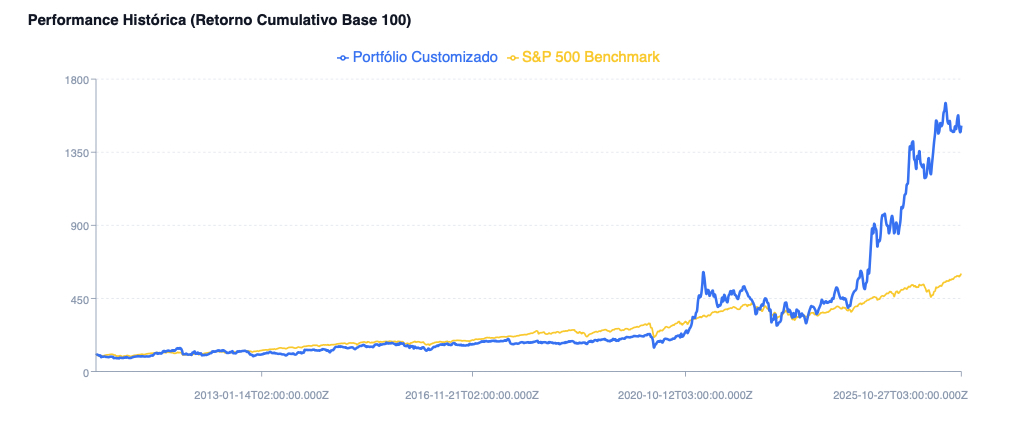
\includegraphics[width=\textwidth]{figuras/perfmediocom.jpg}
   \label{fig:validacao-medio-com-mod}
   \fonte{Elaborado pelos autores.}
\end{figure}

A mudança no resultado é drástica. O portfólio encerra o período próximo do valor 1550, contra os aproximadamente 600 do S\&P 500, superando o \textit{benchmark} em uma razão superior a duas vezes e meia. A aderência entre as duas séries se mantém razoavelmente próxima até aproximadamente 2020, ponto a partir do qual o índice customizado inicia um deslocamento ascendente, com aceleração perceptível nos últimos anos da série e picos que ultrapassam o valor 1600 no fechamento do período.

O contraste entre os dois cenários materializa a proposta central do trabalho no que diz respeito aos modificadores. A fórmula do Risco Modificado, incorpora ao risco base as contribuições padronizadas do EV/EBITDA como amplificador, do \textit{Trailing Dividend Yield} como amplificador e da Margem EBITDA como amortecedor. Ao ativar esses componentes, o cálculo passa a penalizar ativos com múltiplos de \textit{valuation} elevados e dividendos infláveis e a beneficiar ativos com margem operacional robusta.

O resultado deve ser interpretado com uma ressalva metodológica importante. Trata-se de um teste com pesos padrão dos modificadores aplicados retrospectivamente sobre o histórico completo, sem revalidação em janelas de treino e teste separadas. Isto se dá devido a uma limitação da a API utilizada que não disponibiliza os dados institucionais de maneira histórica referente aos ativos. Ainda assim, a magnitude do desempenho observado, obtida com uma configuração de pesos discreta e uniforme, constitui evidência de que a incorporação dos modificadores ao critério de seleção adiciona informação relevante em relação ao uso isolado do risco estatístico, o que fundamenta a defesa do modelo composto como principal contribuição analítica do trabalho.

\subsubsection{Faixa Alto}
\label{subsubsec:validacao-alto}

A Figura~\ref{fig:validacao-alto-padrao} apresenta o resultado do protocolo padrão para a faixa Alto ao longo do horizonte de 2010 a 2025.

\begin{figure}[htb]
   \centering
   \caption{Desempenho histórico do índice customizado da faixa Alto contra o S\&P 500, base 100, período 2010 a 2025, protocolo padrão.}
   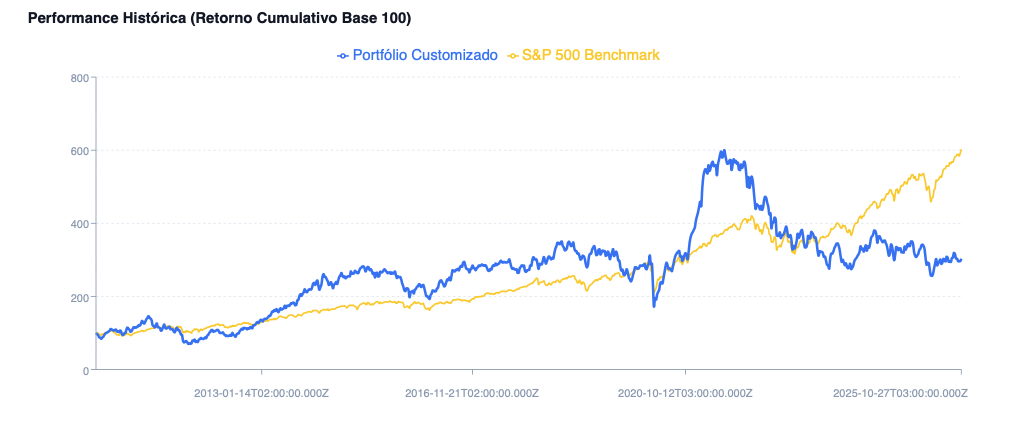
\includegraphics[width=\textwidth]{figuras/perfaltosem.jpg}
   \label{fig:validacao-alto-padrao}
   \fonte{Elaborado pelos autores.}
\end{figure}

O comportamento observado nesta faixa quebra o padrão apresentado anteriormente, com o desempenho do índice inversamente proporcional a seu risco. O portfólio parte ligeiramente à frente do S\&P 500 e mantém liderança até aproximadamente 2023, ponto em que o \textit{benchmark} assume vantagem e a preserva até 2025. Durante o choque pandêmico, o índice customizado exibe uma forte recuperação, ultrapassando o valor 600 em 2021 e assumindo temporariamente uma folga expressiva sobre o \textit{benchmark}, antes de sofrer forte correção nos anos seguintes e encerrar o período próximo do valor 300, contra aproximadamente 600 do S\&P 500. A alternância de liderança e a amplitude das oscilações são compatíveis com a natureza mais volátil da faixa, na qual ativos individuais de perfil mais arriscado tendem a produzir movimentos de maior magnitude.

A Figura~\ref{fig:validacao-alto-setorial} apresenta o resultado dessa variação. Em vez de selecionar as dez ações de maior alocação recomendada dentro do conjunto completo da faixa Alto, o portfólio é composto por nove ativos, distribuídos como as três ações de maior alocação recomendada em cada um dos três setores identificados como os de maior \textit{Z-Score} de risco na análise do painel de Exposição Setorial, discutido na Seção~\ref{subsec:exposicao-setorial}.

\begin{figure}[htb]
   \centering
   \caption{Desempenho histórico do índice customizado da faixa Alto contra o S\&P 500, base 100, período 2010 a 2025, composto por três ações de cada um dos três setores de maior \textit{Z-Score} de risco.}
   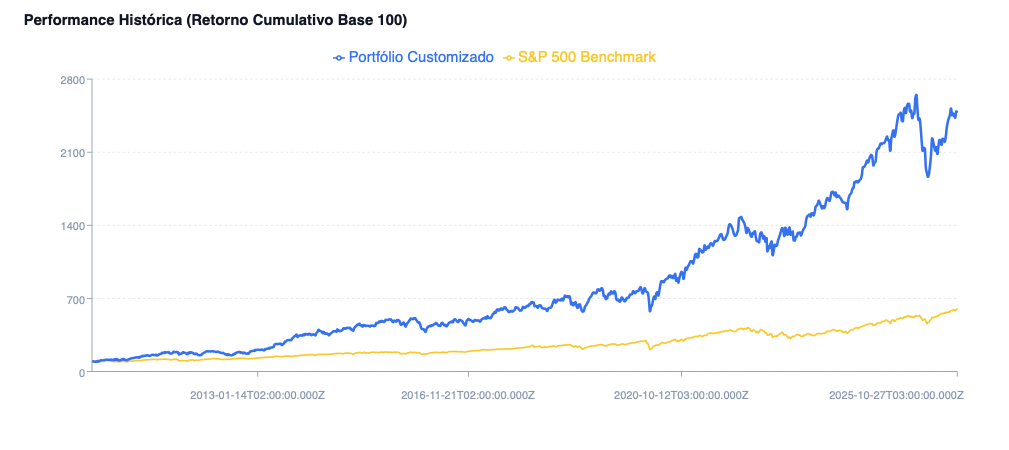
\includegraphics[width=\textwidth]{figuras/perfaltosetor.jpg}
   \label{fig:validacao-alto-setorial}
   \fonte{Elaborado pelos autores.}
\end{figure}

O portfólio encerra o período próximo do valor 2500, superando o S\&P 500 em uma razão superior a quatro vezes no fechamento do horizonte. A trajetória mantém aderência ao \textit{benchmark} durante os primeiros anos da série e passa a se descolar de forma progressiva a partir de 2013, com aceleração acentuada após 2020 e picos que ultrapassam o valor 2600 nos anos finais do período. A magnitude da diferença de desempenho é comparável, em ordem de grandeza, à observada na faixa Médio com modificadores ativados, ainda que obtida por um caminho metodológico distinto. A restrição do conjunto aos três setores de maior \textit{Z-Score} de risco significa selecionar setores nos quais o próprio modelo identifica maior exposição ao risco sistêmico, o que, em conjunto com a escolha da faixa Alto, resulta em um recorte que concentra ativos com maior potencial de oscilação. O portfólio resultante é, portanto, uma composição de ativos de risco elevado mas com fundamentos sólidos dentro de suas respectivas categorias, o que oferece uma explicação plausível para o desempenho superior observado.

Vale a mesma ressalva metodológica apresentada na discussão da faixa Médio. O experimento não separa janelas de treino e teste e utiliza informação de setores agregada sobre o período completo. A relevância do achado, entretanto, é o comportamento comparativo: ao aproveitar a informação produzida por um painel do dashboard para restringir o conjunto de seleção de outro, o modelo composto entrega desempenho muito superior ao obtido pela aplicação isolada de qualquer uma das duas lógicas, o que reforça a leitura do ambiente analítico como um todo integrado, e não como um agregado de consultas independentes. 

\subsubsection{Faixa Muito Alto}
\label{subsubsec:validacao-muito-alto}

A Figura~\ref{fig:validacao-muito-alto} apresenta o resultado do índice customizado composto pelas dez ações de maior alocação recomendada dentro da faixa Muito Alto, no protocolo padrão, ao longo do intervalo de 2010 a 2025.

\begin{figure}[htb]
   \centering
   \caption{Desempenho histórico do índice customizado da faixa Muito Alto contra o S\&P 500, base 100, período 2010 a 2025.}
   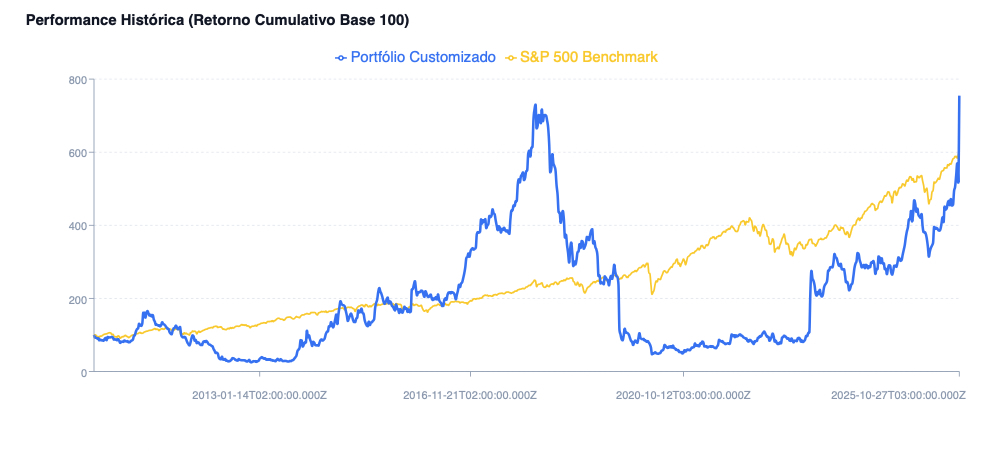
\includegraphics[width=\textwidth]{figuras/perfmuitoaltosem.jpg}
   \label{fig:validacao-muito-alto}
   \fonte{Elaborado pelos autores.}
\end{figure}

O comportamento do portfólio desta faixa é dominado por volatilidade, com amplitudes de oscilação instáveis de desempenho relativo. A trajetória apresenta uma queda inicial nos primeiros anos da série, com o índice recuando para valores próximos de 30 até meados de 2013, seguida por uma grande recuperação que leva o portfólio a ultrapassar o valor 700 em torno de 2017, superando o S\&P 500 no pico. A partir desse ponto, o índice sofre uma correção e retorna a patamares próximos de 100 por volta de 2023, alterna períodos de recuperação parcial e novas quedas ao longo do intervalo pós-pandêmico, e encerra o horizonte próximo do valor 750, novamente à frente do \textit{benchmark} após uma alta acentuada nos meses finais da série.

Observamos que um portfólio que apresenta oscilações da ordem de várias centenas de pontos percentuais em janelas de poucos anos, com fases nas quais perde mais de setenta por cento do valor inicial e fases nas quais multiplica por sete o mesmo valor, não constitui uma proposta de investimento defensável em qualquer critério razoável de avaliação de estratégia. A leitura relevante do painel não é o retorno final, mas justamente a magnitude das oscilações observadas ao longo da série, que corrobora empiricamente a caracterização atribuída pelo modelo à faixa Muito Alto.

Esse comportamento é coerente com os resultados discutidos anteriormente no capítulo. No painel de \textit{Maximum Drawdown}, apresentado na Seção~\ref{subsec:mdd}, a faixa Muito Alto exibiu uma queda próxima a $-85\%$ no recorte de 2010 a 2017 e a $-78\%$ no recorte de 2019 a 2023, valores muito superiores aos das demais faixas e do \textit{benchmark}. No painel de Evolução por Risco, apresentado na Seção~\ref{subsec:painel-evolucao-risco}, o portfólio equiponderado da mesma faixa exibiu desempenho consistentemente inferior ao das demais faixas ao longo de todo o período, permanecendo próximo ao valor 100 durante boa parte do intervalo. O comportamento observado agora, com um portfólio de dez ações selecionadas pela lógica de alocação, alterna picos e vales de magnitude ainda mais acentuada, o que evidencia que a concentração em apenas dez ativos da faixa mais arriscada amplifica as características de risco extremo já identificadas nos painéis anteriores.

\subsubsection{Composição Cruzada por Setor sem Restrição de Faixa}
\label{subsubsec:validacao-cruzada-setor}

As cinco discussões anteriores mantiveram a faixa de risco como critério inicial de recorte do conjunto de seleção. O painel de Teste de Alocação, entretanto, não impõe essa restrição: nada impede o usuário de compor um índice customizado a partir de ativos originados de faixas ou setores distintos, desde que ambos apareçam entre as maiores alocações recomendadas dentro dos critérios ativos. Esta subseção apresenta um exemplo dessa flexibilidade, mostrando que a lógica de composição pode ser orientada por outros princípios analíticos além da estratificação por faixa.

A composição adotada parte da leitura do painel de Exposição Setorial, discutido na Seção~\ref{subsec:exposicao-setorial}, no qual \textit{Industrials} e \textit{Real Estate} apareceram em posições aproximadamente simétricas em torno do eixo neutro do \textit{Z-Score} setorial, o primeiro ligeiramente acima de zero e o segundo ligeiramente abaixo, ambos com magnitudes semelhantes. A hipótese explorada é que ativos originados de setores com \textit{scores} de risco simétricos e de baixa magnitude podem produzir, quando combinados, um portfólio no qual o risco sistêmico de cada setor tende a se compensar parcialmente. Para verificar essa hipótese, foi selecionada a combinação das cinco ações de maior alocação recomendada em \textit{Industrials} com as cinco ações de maior alocação recomendada em \textit{Real Estate}, sem qualquer filtro adicional por faixa de risco.

\begin{figure}[htb]
   \centering
   \caption{Desempenho histórico do índice customizado composto pelas cinco maiores alocações de \textit{Industrials} e pelas cinco maiores alocações de \textit{Real Estate} contra o S\&P 500, base 100, período 2010 a 2025.}
   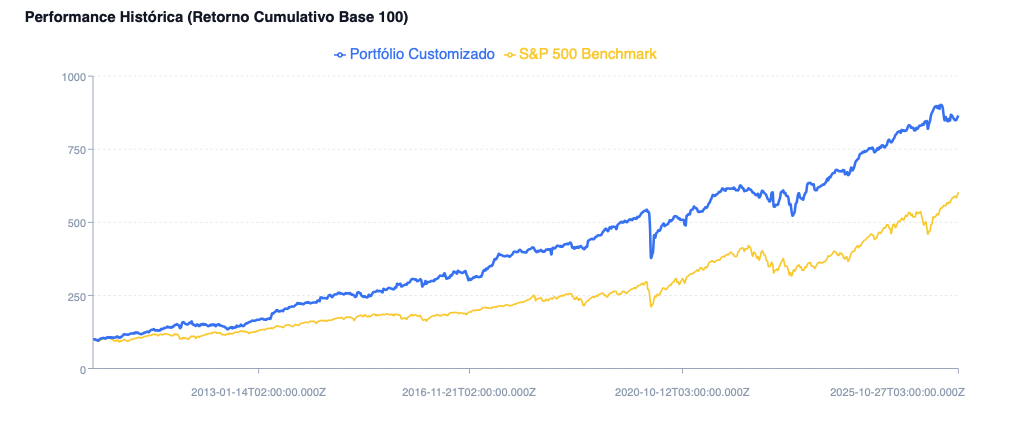
\includegraphics[width=\textwidth]{figuras/perfbalanceadosetor.jpg}
   \label{fig:validacao-cruzada-setor}
   \fonte{Elaborado pelos autores.}
\end{figure}

A Figura~\ref{fig:validacao-cruzada-setor} apresenta o resultado do índice customizado assim composto ao longo do horizonte de 2010 a 2025. O portfólio encerra o período próximo do valor 850, contra aproximadamente 600 do S\&P 500 no mesmo marco temporal, e mantém-se à frente do \textit{benchmark} ao longo de praticamente todo o período. A trajetória apresenta perfil substancialmente mais estável que o observado na faixa Muito Alto discutida na Seção~\ref{subsubsec:validacao-muito-alto} e revela oscilações mais suaves que as das faixas Médio e Alto quando essas foram testadas em suas variações de melhor desempenho. Os principais eventos macroeconômicos do intervalo, notadamente o choque pandêmico de 2020, aparecem como vales localizados na série, seguidos por retomada consistente da tendência de alta.

O resultado reforça a capacidade do ambiente analítico de unir informações adquiridas em painéis distintos no estudo de novos índices. As cinco composições anteriores exploraram a estratificação por faixa de risco como eixo principal de análise, e a variação apresentada na Seção~\ref{subsubsec:validacao-alto} já havia demonstrado o valor de cruzar essa estratificação com o ranqueamento setorial. A composição desta subseção avança um passo adicional na mesma direção, prescindindo completamente do recorte por faixa e utilizando exclusivamente a leitura setorial como critério de balanceamento. A capacidade de sustentar essa variedade de protocolos analíticos sobre a mesma base de dados e a mesma interface alinha-se ao objetivo geral de construir um ambiente integrado no qual as consultas dialogam entre si para viabilizar análises que nenhuma delas isoladamente permitiria.

\section{Resultados Finais}
\label{sec:resultados-todo}

As três seções anteriores exploraram o ambiente analítico segundo eixos distintos de leitura sobre o mesmo universo de ações. A Seção~\ref{sec:consultas-setor} tratou o mercado a partir da agregação por setor econômico, a Seção~\ref{sec:evolucao-risco} organizou as ações em faixas simétricas derivadas do risco base padronizado, e a Seção~\ref{sec:consultas-alocacao} operacionalizou a lógica de composição de índices customizados confrontados ao S\&P~500. Esta seção retoma essas leituras em conjunto, evidencia as convergências e especificidades entre elas e discute o significado dos achados diante do objetivo declarado no Capítulo~\ref{introducao}.

O eixo setorial revelou que a estrutura de retorno, volatilidade e correlação do mercado americano no período analisado é dominada por um \textit{cluster} central de setores fortemente correlacionados, no qual \textit{Consumer Cyclical, Industrials, Technology, Utilities e Consumer Defensive} se movem de forma sincronizada, enquanto \textit{Energy} e \textit{Real Estate} se comportam como diversificadores por razões distintas, o primeiro por sua resposta contrária a choques inflacionários e o segundo por seu ciclo específico de sensibilidade a juros. O eixo de risco mostrou que a estratificação por Z-Score aplicada ao risco base produz uma escala coerente com o comportamento esperado do mercado em janelas longas, com hierarquia preservada em retorno anualizado e separação nítida da faixa Muito Alto no \textit{maximum drawdown}, ainda que o poder discriminante entre as faixas centrais se comprima em janelas curtas ou dominadas por choques sistêmicos. O eixo de alocação demonstrou que a lógica de ponderação exponencial sobre o Z-Score de qualidade viabiliza a construção de índices customizados cuja trajetória histórica pode ser lida como aderente, superior ou inferior ao S\&P~500 conforme a combinação de critérios adotada.

Uma convergência relevante entre os três eixos aparece na leitura do paradoxo da baixa volatilidade. O painel de Evolução por Risco, discutido na Seção~\ref{subsec:painel-evolucao-risco}, sinalizou o fenômeno pela via da comparação entre portfólios equiponderados por faixa. O painel de Teste de Alocação, discutido na Seção~\ref{sec:tabela-alocacao}, o reproduziu pela via da comparação entre índices customizados construídos por critério de qualidade dentro de cada faixa. O painel de Exposição Setorial, discutido na Seção~\ref{subsec:exposicao-setorial}, forneceu a leitura estrutural do fenômeno ao mostrar que setores defensivos ocupam consistentemente a região negativa do Z-Score de risco. As três leituras se reforçam mutuamente e sustentam, dentro do universo analisado, a interpretação de que risco estatístico mais elevado não se traduz automaticamente em retorno médio superior, apesar de a hierarquia se preservar no acumulado suficientemente longo.

A especificidade de cada eixo também merece registro. O eixo setorial produziu leituras difíceis de obter apenas com o critério de risco, notadamente a identificação de setores diversificadores e a caracterização sazonal dos retornos mensais. O eixo de risco produziu uma classificação de ativos que serve de insumo à lógica de alocação e viabiliza a comparação por faixa entre carteiras. O eixo de alocação possibilitou o cruzamento entre os dois primeiros na construção de índices customizados, e apenas nele foi possível observar o efeito da ativação dos modificadores propostos no modelo composto e o ganho de desempenho derivado da restrição por setores de maior Z-Score de risco, discutido na Seção~\ref{subsubsec:validacao-alto}. A composição cruzada apresentada na Seção~\ref{subsubsec:validacao-cruzada-setor}, por sua vez, mostrou que a abordagem sustenta protocolos analíticos que prescindem da estratificação por faixa e utilizam exclusivamente informação setorial como critério de balanceamento.

O objetivo geral declarado no Capítulo~\ref{introducao} não se limitava à proposição de novos indicadores de risco, mas visava a construção de um ambiente analítico integrado no qual coleta, tratamento, modelagem dimensional e composição de métricas operassem como um sistema único, orientado à viabilização de análises complexas, e os resultados aqui apresentados sustentam essa proposta. Em primeiro lugar, o conjunto de leituras discutidas ao longo do capítulo não seria obtido pela consulta a índices tradicionais isolados, uma vez que estes operam sob ponderação por valor de mercado, restringem a comparação a agregados fixos e não expõem ao usuário nem os critérios de composição nem os mecanismos de estratificação por risco. Além disso, a comparação sistemática contra o S\&P~500 foi viabilizada pela mesma base de dados e pela mesma interface, o que assegura homogeneidade metodológica entre as leituras. E também, a interatividade dos painéis permite ao usuário alterar filtros, janelas temporais, pesos dos modificadores e composição dos índices customizados sem qualquer intervenção sobre a camada de dados, o que é a evidência prática de que o ambiente entrega flexibilidade além do escopo de uma consulta pontual.

Os objetivos específicos declarados no Capítulo~\ref{introducao} podem ser mapeados diretamente aos resultados evidenciados neste capítulo. A identificação das fontes de dados e a modelagem conceitual materializaram-se na disponibilidade completa do universo de 2010 a 2025 sobre o qual todas as consultas operam, e sem essa base os quatro painéis setoriais discutidos na Seção~\ref{sec:consultas-setor} não seriam sustentáveis. A implementação do pipeline de transformação de dados evidencia-se na consistência dos indicadores calculados exibidos no painel de Listagem de Ações, discutido na Seção~\ref{subsec:painel-listagem}, e na materialização da coluna de faixa de risco utilizada em todos os painéis da Seção~\ref{sec:evolucao-risco}. A construção e aplicação das métricas quantitativas de risco evidenciam-se nos resultados dos painéis de Retorno Anualizado, \textit{Maximum Drawdown} e Exposição Setorial, discutidos nas Seções~\ref{subsec:retorno-por-faixa}, \ref{subsec:mdd} e \ref{subsec:exposicao-setorial}. 

O balanço dos resultados revela robustez e fragilidade em pontos distintos. A robustez aparece com maior clareza na estabilidade da estrutura setorial, na identificação consistente da faixa Muito Alto como zona de risco extremo em qualquer janela analisada, na preservação do paradoxo da baixa volatilidade em leituras metodologicamente independentes e no ganho de desempenho observado no cruzamento entre estratificação por risco e restrição setorial. A fragilidade aparece de forma com a impossibilidade de revalidação em janelas de treino e teste separadas para os modificadores do modelo composto, decorrente da natureza estática dos dados institucionais disponibilizados pela API.

As ressalvas metodológicas consolidadas discutidas anteriormente devem ser lidas em conjunto com esse balanço. Nenhum dos resultados aqui reportados constitui prova estatística de superioridade de estratégia, tampouco recomendação de investimento. O que os resultados sustentam é que o ambiente analítico entregou análises coerentes, replicáveis sob diferentes recortes e capazes de dialogar entre painéis, e que essas análises revelaram fenômenos de mercado alinhados à literatura de finanças quantitativas\footnote{O código-fonte completo do ambiente analítico está disponível em \url{https://github.com/0nerb/TCC}.}.